\documentclass[1p]{elsarticle_modified}
%\bibliographystyle{elsarticle-num}

%\usepackage[colorlinks]{hyperref}
%\usepackage{abbrmath_seonhwa} %\Abb, \Ascr, \Acal ,\Abf, \Afrak
\usepackage{amsfonts}
\usepackage{amssymb}
\usepackage{amsmath}
\usepackage{amsthm}
\usepackage{scalefnt}
\usepackage{amsbsy}
\usepackage{kotex}
\usepackage{caption}
\usepackage{subfig}
\usepackage{color}
\usepackage{graphicx}
\usepackage{xcolor} %% white, black, red, green, blue, cyan, magenta, yellow
\usepackage{float}
\usepackage{setspace}
\usepackage{hyperref}

\usepackage{tikz}
\usetikzlibrary{arrows}

\usepackage{multirow}
\usepackage{array} % fixed length table
\usepackage{hhline}

%%%%%%%%%%%%%%%%%%%%%
\makeatletter
\renewcommand*\env@matrix[1][\arraystretch]{%
	\edef\arraystretch{#1}%
	\hskip -\arraycolsep
	\let\@ifnextchar\new@ifnextchar
	\array{*\c@MaxMatrixCols c}}
\makeatother %https://tex.stackexchange.com/questions/14071/how-can-i-increase-the-line-spacing-in-a-matrix
%%%%%%%%%%%%%%%

\usepackage[normalem]{ulem}

\newcommand{\msout}[1]{\ifmmode\text{\sout{\ensuremath{#1}}}\else\sout{#1}\fi}
%SOURCE: \msout is \stkout macro in https://tex.stackexchange.com/questions/20609/strikeout-in-math-mode

\newcommand{\cancel}[1]{
	\ifmmode
	{\color{red}\msout{#1}}
	\else
	{\color{red}\sout{#1}}
	\fi
}

\newcommand{\add}[1]{
	{\color{blue}\uwave{#1}}
}

\newcommand{\replace}[2]{
	\ifmmode
	{\color{red}\msout{#1}}{\color{blue}\uwave{#2}}
	\else
	{\color{red}\sout{#1}}{\color{blue}\uwave{#2}}
	\fi
}

\newcommand{\Sol}{\mathcal{S}} %segment
\newcommand{\D}{D} %diagram
\newcommand{\A}{\mathcal{A}} %arc


%%%%%%%%%%%%%%%%%%%%%%%%%%%%%5 test

\def\sl{\operatorname{\textup{SL}}(2,\Cbb)}
\def\psl{\operatorname{\textup{PSL}}(2,\Cbb)}
\def\quan{\mkern 1mu \triangleright \mkern 1mu}

\theoremstyle{definition}
\newtheorem{thm}{Theorem}[section]
\newtheorem{prop}[thm]{Proposition}
\newtheorem{lem}[thm]{Lemma}
\newtheorem{ques}[thm]{Question}
\newtheorem{cor}[thm]{Corollary}
\newtheorem{defn}[thm]{Definition}
\newtheorem{exam}[thm]{Example}
\newtheorem{rmk}[thm]{Remark}
\newtheorem{alg}[thm]{Algorithm}

\newcommand{\I}{\sqrt{-1}}
\begin{document}

%\begin{frontmatter}
%
%\title{Boundary parabolic representations of knots up to 8 crossings}
%
%%% Group authors per affiliation:
%\author{Yunhi Cho} 
%\address{Department of Mathematics, University of Seoul, Seoul, Korea}
%\ead{yhcho@uos.ac.kr}
%
%
%\author{Seonhwa Kim} %\fnref{s_kim}}
%\address{Center for Geometry and Physics, Institute for Basic Science, Pohang, 37673, Korea}
%\ead{ryeona17@ibs.re.kr}
%
%\author{Hyuk Kim}
%\address{Department of Mathematical Sciences, Seoul National University, Seoul 08826, Korea}
%\ead{hyukkim@snu.ac.kr}
%
%\author{Seokbeom Yoon}
%\address{Department of Mathematical Sciences, Seoul National University, Seoul, 08826,  Korea}
%\ead{sbyoon15@snu.ac.kr}
%
%\begin{abstract}
%We find all boundary parabolic representation of knots up to 8 crossings.
%
%\end{abstract}
%\begin{keyword}
%    \MSC[2010] 57M25 
%\end{keyword}
%
%\end{frontmatter}

%\linenumbers
%\tableofcontents
%
\newcommand\colored[1]{\textcolor{white}{\rule[-0.35ex]{0.8em}{1.4ex}}\kern-0.8em\color{red} #1}%
%\newcommand\colored[1]{\textcolor{white}{ #1}\kern-2.17ex	\textcolor{white}{ #1}\kern-1.81ex	\textcolor{white}{ #1}\kern-2.15ex\color{red}#1	}

{\Large $\underline{12a_{0472}~(K12a_{0472})}$}

\setlength{\tabcolsep}{10pt}
\renewcommand{\arraystretch}{1.6}
\vspace{1cm}\begin{tabular}{m{100pt}>{\centering\arraybackslash}m{274pt}}
\multirow{5}{120pt}{
	\centering
	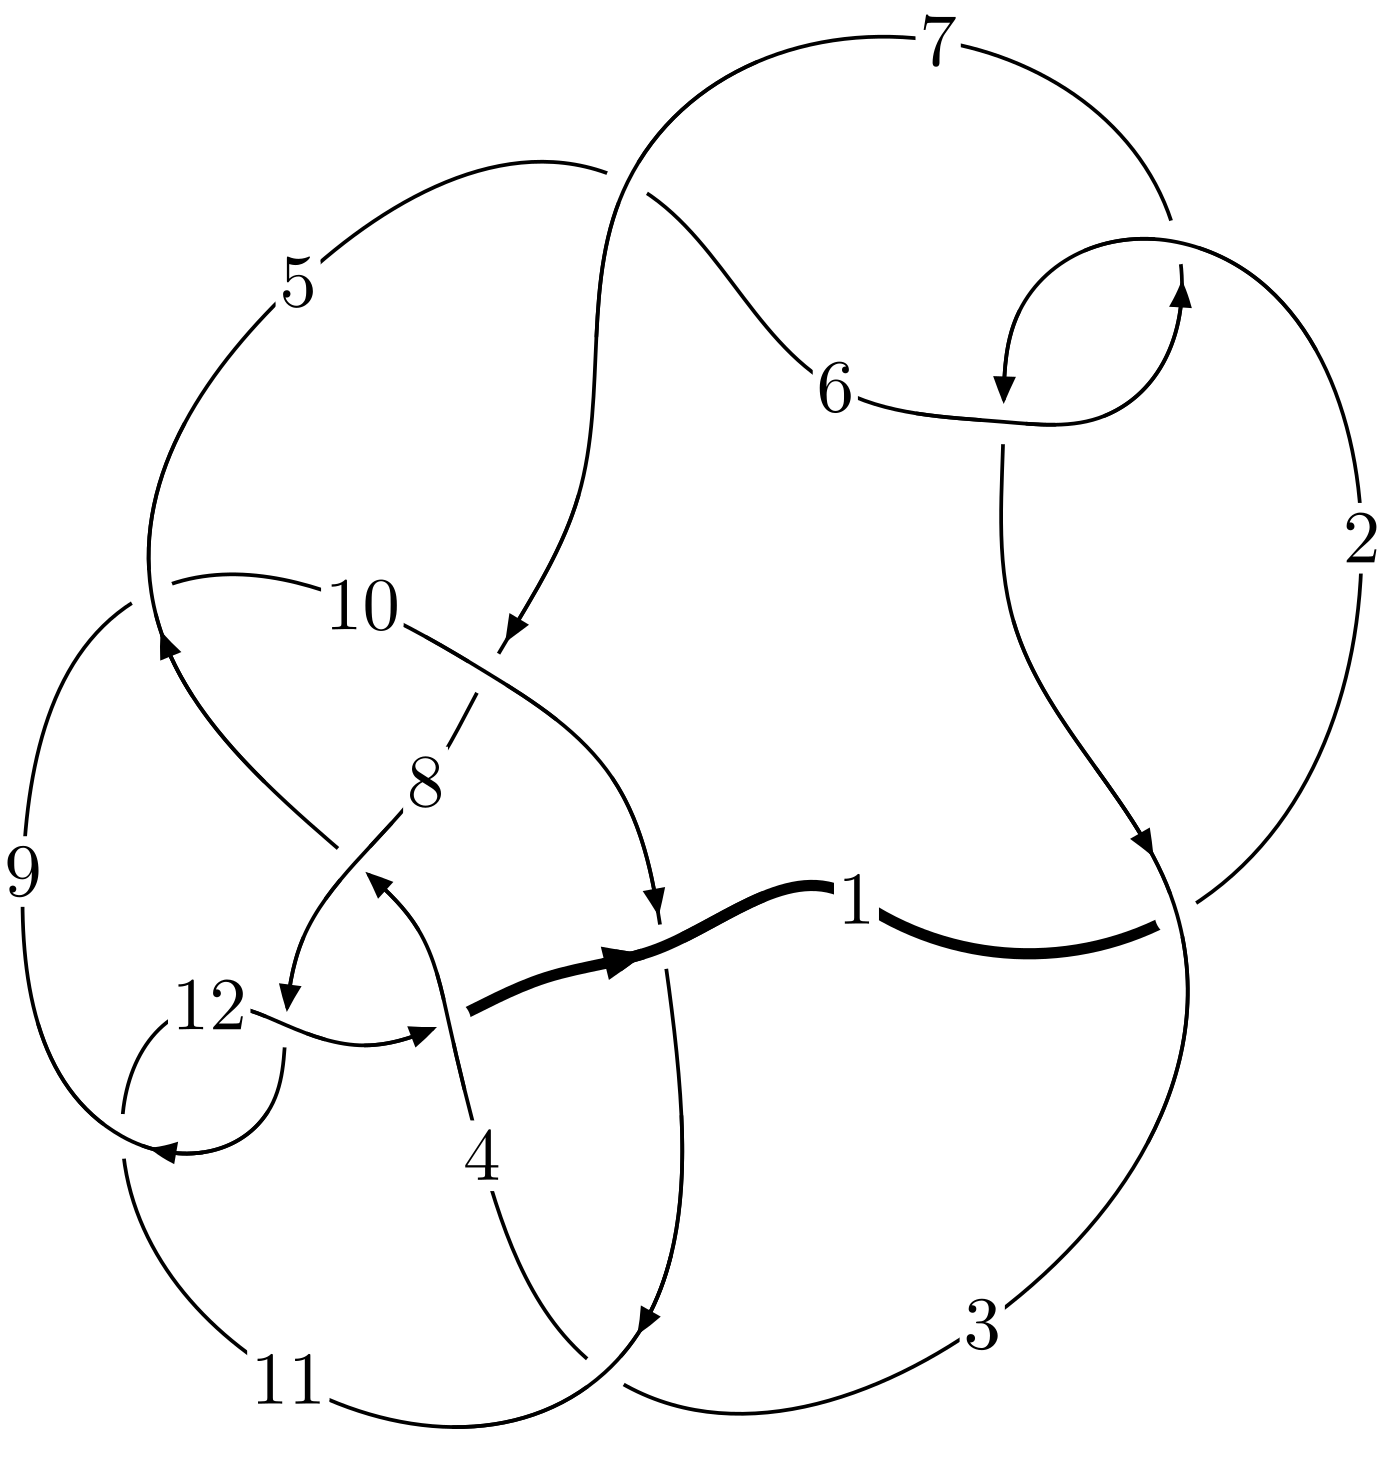
\includegraphics[width=112pt]{../../../GIT/diagram.site/Diagrams/png/1273_12a_0472.png}\\
\ \ \ A knot diagram\footnotemark}&
\allowdisplaybreaks
\textbf{Linearized knot diagam} \\
\cline{2-2}
 &
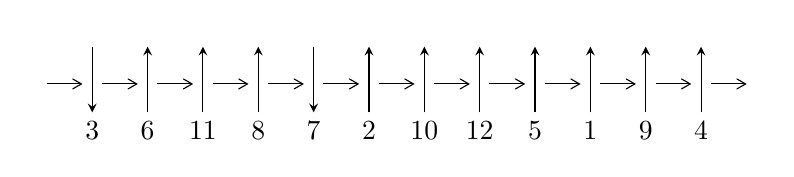
\begin{tikzpicture}[x=20pt, y=17pt]
	% nodes
	\node (C0) at (0, 0) {};
	\node (C1) at (1, 0) {};
	\node (C1U) at (1, +1) {};
	\node (C1D) at (1, -1) {3};

	\node (C2) at (2, 0) {};
	\node (C2U) at (2, +1) {};
	\node (C2D) at (2, -1) {6};

	\node (C3) at (3, 0) {};
	\node (C3U) at (3, +1) {};
	\node (C3D) at (3, -1) {11};

	\node (C4) at (4, 0) {};
	\node (C4U) at (4, +1) {};
	\node (C4D) at (4, -1) {8};

	\node (C5) at (5, 0) {};
	\node (C5U) at (5, +1) {};
	\node (C5D) at (5, -1) {7};

	\node (C6) at (6, 0) {};
	\node (C6U) at (6, +1) {};
	\node (C6D) at (6, -1) {2};

	\node (C7) at (7, 0) {};
	\node (C7U) at (7, +1) {};
	\node (C7D) at (7, -1) {10};

	\node (C8) at (8, 0) {};
	\node (C8U) at (8, +1) {};
	\node (C8D) at (8, -1) {12};

	\node (C9) at (9, 0) {};
	\node (C9U) at (9, +1) {};
	\node (C9D) at (9, -1) {5};

	\node (C10) at (10, 0) {};
	\node (C10U) at (10, +1) {};
	\node (C10D) at (10, -1) {1};

	\node (C11) at (11, 0) {};
	\node (C11U) at (11, +1) {};
	\node (C11D) at (11, -1) {9};

	\node (C12) at (12, 0) {};
	\node (C12U) at (12, +1) {};
	\node (C12D) at (12, -1) {4};
	\node (C13) at (13, 0) {};

	% arrows
	\draw[->,>={angle 60}]
	(C0) edge (C1) (C1) edge (C2) (C2) edge (C3) (C3) edge (C4) (C4) edge (C5) (C5) edge (C6) (C6) edge (C7) (C7) edge (C8) (C8) edge (C9) (C9) edge (C10) (C10) edge (C11) (C11) edge (C12) (C12) edge (C13) ;	\draw[->,>=stealth]
	(C1U) edge (C1D) (C2D) edge (C2U) (C3D) edge (C3U) (C4D) edge (C4U) (C5U) edge (C5D) (C6D) edge (C6U) (C7D) edge (C7U) (C8D) edge (C8U) (C9D) edge (C9U) (C10D) edge (C10U) (C11D) edge (C11U) (C12D) edge (C12U) ;
	\end{tikzpicture} \\
\hhline{~~} \\& 
\textbf{Solving Sequence} \\ \cline{2-2} 
 &
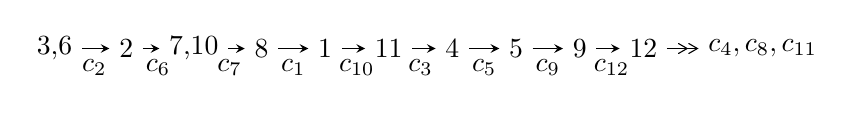
\begin{tikzpicture}[x=23pt, y=7pt]
	% node
	\node (A0) at (-1/8, 0) {3,6};
	\node (A1) at (1, 0) {2};
	\node (A2) at (33/16, 0) {7,10};
	\node (A3) at (25/8, 0) {8};
	\node (A4) at (33/8, 0) {1};
	\node (A5) at (41/8, 0) {11};
	\node (A6) at (49/8, 0) {4};
	\node (A7) at (57/8, 0) {5};
	\node (A8) at (65/8, 0) {9};
	\node (A9) at (73/8, 0) {12};
	\node (C1) at (1/2, -1) {$c_{2}$};
	\node (C2) at (3/2, -1) {$c_{6}$};
	\node (C3) at (21/8, -1) {$c_{7}$};
	\node (C4) at (29/8, -1) {$c_{1}$};
	\node (C5) at (37/8, -1) {$c_{10}$};
	\node (C6) at (45/8, -1) {$c_{3}$};
	\node (C7) at (53/8, -1) {$c_{5}$};
	\node (C8) at (61/8, -1) {$c_{9}$};
	\node (C9) at (69/8, -1) {$c_{12}$};
	\node (A10) at (11, 0) {$c_{4},c_{8},c_{11}$};

	% edge
	\draw[->,>=stealth]	
	(A0) edge (A1) (A1) edge (A2) (A2) edge (A3) (A3) edge (A4) (A4) edge (A5) (A5) edge (A6) (A6) edge (A7) (A7) edge (A8) (A8) edge (A9) ;
	\draw[->>,>={angle 60}]	
	(A9) edge (A10);
\end{tikzpicture} \\ 

\end{tabular} \\

\footnotetext{
The image of knot diagram is generated by the software ``\textbf{Draw programme}" developed by Andrew Bartholomew(\url{http://www.layer8.co.uk/maths/draw/index.htm\#Running-draw}), where we modified some parts for our purpose(\url{https://github.com/CATsTAILs/LinksPainter}).
}\phantom \\ \newline 
\centering \textbf{Ideals for irreducible components\footnotemark of $X_{\text{par}}$} 
 
\begin{align*}
I^u_{1}&=\langle 
-3.80673\times10^{16} u^{62}-2.40994\times10^{17} u^{61}+\cdots+6.68228\times10^{14} b+5.92854\times10^{17},\\
\phantom{I^u_{1}}&\phantom{= \langle  }5.92854\times10^{17} u^{62}+6.30921\times10^{18} u^{61}+\cdots+6.68228\times10^{15} a+9.39437\times10^{18},\\
\phantom{I^u_{1}}&\phantom{= \langle  }u^{63}+10 u^{62}+\cdots+26 u+10\rangle \\
I^u_{2}&=\langle 
- u^{42}-2 u^{41}+\cdots+2 b-10,\;-10 u^{42} a+10 u^{42}+\cdots+13 a-27,\;u^{43}-3 u^{42}+\cdots+5 u^2+1\rangle \\
I^u_{3}&=\langle 
2 u^{22}+16 u^{21}+\cdots+b+31,\;-31 u^{22}+97 u^{21}+\cdots+2 a+74,\;u^{23}-3 u^{22}+\cdots-2 u+2\rangle \\
I^u_{4}&=\langle 
a^3 u- a^3- a^2 u+a^2+6 a u+3 b+3 a- u+1,\;a^4-3 a^2 u- a^2-2 a u-2 a-2 u-2,\;u^2+u+1\rangle \\
\\
\end{align*}
\raggedright * 4 irreducible components of $\dim_{\mathbb{C}}=0$, with total 180 representations.\\
\footnotetext{All coefficients of polynomials are rational numbers. But the coefficients are sometimes approximated in decimal forms when there is not enough margin.}
\newpage
\renewcommand{\arraystretch}{1}
\centering \section*{I. $I^u_{1}= \langle -3.81\times10^{16} u^{62}-2.41\times10^{17} u^{61}+\cdots+6.68\times10^{14} b+5.93\times10^{17},\;5.93\times10^{17} u^{62}+6.31\times10^{18} u^{61}+\cdots+6.68\times10^{15} a+9.39\times10^{18},\;u^{63}+10 u^{62}+\cdots+26 u+10 \rangle$}
\flushleft \textbf{(i) Arc colorings}\\
\begin{tabular}{m{7pt} m{180pt} m{7pt} m{180pt} }
\flushright $a_{3}=$&$\begin{pmatrix}1\\0\end{pmatrix}$ \\
\flushright $a_{6}=$&$\begin{pmatrix}0\\u\end{pmatrix}$ \\
\flushright $a_{2}=$&$\begin{pmatrix}1\\u^2\end{pmatrix}$ \\
\flushright $a_{7}=$&$\begin{pmatrix}u\\u^3+u\end{pmatrix}$ \\
\flushright $a_{10}=$&$\begin{pmatrix}-88.7203 u^{62}-944.171 u^{61}+\cdots-2753.65 u-1405.86\\56.9675 u^{62}+360.646 u^{61}+\cdots-900.864 u-887.203\end{pmatrix}$ \\
\flushright $a_{8}=$&$\begin{pmatrix}19.0481 u^{62}+241.655 u^{61}+\cdots+1061.36 u+631.264\\-51.1743 u^{62}-411.730 u^{61}+\cdots-135.013 u+190.481\end{pmatrix}$ \\
\flushright $a_{1}=$&$\begin{pmatrix}u^2+1\\u^2\end{pmatrix}$ \\
\flushright $a_{11}=$&$\begin{pmatrix}-41.9861 u^{62}-384.463 u^{61}+\cdots-676.460 u-233.296\\11.6546 u^{62}+53.7990 u^{61}+\cdots-419.518 u-348.043\end{pmatrix}$ \\
\flushright $a_{4}=$&$\begin{pmatrix}36.7915 u^{62}+341.158 u^{61}+\cdots+606.220 u+216.945\\30.2923 u^{62}+321.272 u^{61}+\cdots+973.954 u+507.932\end{pmatrix}$ \\
\flushright $a_{5}=$&$\begin{pmatrix}u^3\\u^5+u^3+u\end{pmatrix}$ \\
\flushright $a_{9}=$&$\begin{pmatrix}-51.9436 u^{62}-525.909 u^{61}+\cdots-1320.98 u-613.500\\27.9487 u^{62}+173.947 u^{61}+\cdots-497.766 u-483.244\end{pmatrix}$ \\
\flushright $a_{12}=$&$\begin{pmatrix}-18.0981 u^{62}-158.934 u^{61}+\cdots-263.436 u-62.0849\\19.5842 u^{62}+181.155 u^{61}+\cdots+283.762 u+67.1158\end{pmatrix}$\\&\end{tabular}
\flushleft \textbf{(ii) Obstruction class $= -1$}\\~\\
\flushleft \textbf{(iii) Cusp Shapes $= \frac{289193695666494042}{668227596996943} u^{62}+\frac{2659979644074475993}{668227596996943} u^{61}+\cdots+\frac{4339716891634397392}{668227596996943} u+\frac{1553531502950905056}{668227596996943}$}\\~\\
\newpage\renewcommand{\arraystretch}{1}
\flushleft \textbf{(iv) u-Polynomials at the component}\newline \\
\begin{tabular}{m{50pt}|m{274pt}}
Crossings & \hspace{64pt}u-Polynomials at each crossing \\
\hline $$\begin{aligned}c_{1},c_{5}\end{aligned}$$&$\begin{aligned}
&u^{63}+18 u^{62}+\cdots-444 u-100
\end{aligned}$\\
\hline $$\begin{aligned}c_{2},c_{6}\end{aligned}$$&$\begin{aligned}
&u^{63}-10 u^{62}+\cdots+26 u-10
\end{aligned}$\\
\hline $$\begin{aligned}c_{3},c_{9}\end{aligned}$$&$\begin{aligned}
&u^{63}- u^{62}+\cdots+40 u-19
\end{aligned}$\\
\hline $$\begin{aligned}c_{4},c_{12}\end{aligned}$$&$\begin{aligned}
&u^{63}+3 u^{62}+\cdots+6 u-1
\end{aligned}$\\
\hline $$\begin{aligned}c_{7},c_{10}\end{aligned}$$&$\begin{aligned}
&u^{63}+3 u^{62}+\cdots+6 u-1
\end{aligned}$\\
\hline $$\begin{aligned}c_{8},c_{11}\end{aligned}$$&$\begin{aligned}
&u^{63}+15 u^{62}+\cdots-1262 u-50
\end{aligned}$\\
\hline
\end{tabular}\\~\\
\newpage\renewcommand{\arraystretch}{1}
\flushleft \textbf{(v) Riley Polynomials at the component}\newline \\
\begin{tabular}{m{50pt}|m{274pt}}
Crossings & \hspace{64pt}Riley Polynomials at each crossing \\
\hline $$\begin{aligned}c_{1},c_{5}\end{aligned}$$&$\begin{aligned}
&y^{63}+58 y^{62}+\cdots+948336 y-10000
\end{aligned}$\\
\hline $$\begin{aligned}c_{2},c_{6}\end{aligned}$$&$\begin{aligned}
&y^{63}+18 y^{62}+\cdots-444 y-100
\end{aligned}$\\
\hline $$\begin{aligned}c_{3},c_{9}\end{aligned}$$&$\begin{aligned}
&y^{63}-17 y^{62}+\cdots+8174 y-361
\end{aligned}$\\
\hline $$\begin{aligned}c_{4},c_{12}\end{aligned}$$&$\begin{aligned}
&y^{63}+51 y^{62}+\cdots-106 y-1
\end{aligned}$\\
\hline $$\begin{aligned}c_{7},c_{10}\end{aligned}$$&$\begin{aligned}
&y^{63}+11 y^{62}+\cdots-4 y-1
\end{aligned}$\\
\hline $$\begin{aligned}c_{8},c_{11}\end{aligned}$$&$\begin{aligned}
&y^{63}+31 y^{62}+\cdots+249244 y-2500
\end{aligned}$\\
\hline
\end{tabular}\\~\\
\newpage\flushleft \textbf{(vi) Complex Volumes and Cusp Shapes}
$$\begin{array}{c|c|c}  
\text{Solutions to }I^u_{1}& \I (\text{vol} + \sqrt{-1}CS) & \text{Cusp shape}\\
 \hline 
\begin{aligned}
u &= \phantom{-}0.214740 + 0.981355 I \\
a &= -0.198641 - 0.968427 I \\
b &= -0.907715 + 0.402897 I\end{aligned}
 & -7.36523 + 3.21246 I & \phantom{-0.000000 } 0 \\ \hline\begin{aligned}
u &= \phantom{-}0.214740 - 0.981355 I \\
a &= -0.198641 + 0.968427 I \\
b &= -0.907715 - 0.402897 I\end{aligned}
 & -7.36523 - 3.21246 I & \phantom{-0.000000 } 0 \\ \hline\begin{aligned}
u &= \phantom{-}0.374009 + 0.963149 I \\
a &= -0.568883 + 0.321223 I \\
b &= \phantom{-}0.522153 + 0.427779 I\end{aligned}
 & -6.48970 + 2.46067 I & \phantom{-0.000000 } 0 \\ \hline\begin{aligned}
u &= \phantom{-}0.374009 - 0.963149 I \\
a &= -0.568883 - 0.321223 I \\
b &= \phantom{-}0.522153 - 0.427779 I\end{aligned}
 & -6.48970 - 2.46067 I & \phantom{-0.000000 } 0 \\ \hline\begin{aligned}
u &= -0.299758 + 0.918244 I \\
a &= -0.445543 - 0.542182 I \\
b &= -0.631410 + 0.246594 I\end{aligned}
 & -1.73788 - 2.23954 I & \phantom{-0.000000 } 0 \\ \hline\begin{aligned}
u &= -0.299758 - 0.918244 I \\
a &= -0.445543 + 0.542182 I \\
b &= -0.631410 - 0.246594 I\end{aligned}
 & -1.73788 + 2.23954 I & \phantom{-0.000000 } 0 \\ \hline\begin{aligned}
u &= \phantom{-}0.155216 + 1.032550 I \\
a &= \phantom{-}0.281341 - 0.492123 I \\
b &= -0.551808 - 0.214112 I\end{aligned}
 & -3.10710 - 1.65886 I & \phantom{-0.000000 } 0 \\ \hline\begin{aligned}
u &= \phantom{-}0.155216 - 1.032550 I \\
a &= \phantom{-}0.281341 + 0.492123 I \\
b &= -0.551808 + 0.214112 I\end{aligned}
 & -3.10710 + 1.65886 I & \phantom{-0.000000 } 0 \\ \hline\begin{aligned}
u &= -0.614389 + 0.883223 I \\
a &= -1.400550 + 0.059590 I \\
b &= -0.80785 + 1.27361 I\end{aligned}
 & -1.53239 - 1.91777 I & \phantom{-0.000000 } 0 \\ \hline\begin{aligned}
u &= -0.614389 - 0.883223 I \\
a &= -1.400550 - 0.059590 I \\
b &= -0.80785 - 1.27361 I\end{aligned}
 & -1.53239 + 1.91777 I & \phantom{-0.000000 } 0\\
 \hline 
 \end{array}$$\newpage$$\begin{array}{c|c|c}  
\text{Solutions to }I^u_{1}& \I (\text{vol} + \sqrt{-1}CS) & \text{Cusp shape}\\
 \hline 
\begin{aligned}
u &= -0.672802 + 0.858411 I \\
a &= -0.13281 + 2.03041 I \\
b &= \phantom{-}1.65357 + 1.48007 I\end{aligned}
 & -1.46510 - 3.14067 I & \phantom{-0.000000 } 0 \\ \hline\begin{aligned}
u &= -0.672802 - 0.858411 I \\
a &= -0.13281 - 2.03041 I \\
b &= \phantom{-}1.65357 - 1.48007 I\end{aligned}
 & -1.46510 + 3.14067 I & \phantom{-0.000000 } 0 \\ \hline\begin{aligned}
u &= \phantom{-}0.331456 + 1.046790 I \\
a &= \phantom{-}0.081594 + 0.703396 I \\
b &= \phantom{-}0.709261 - 0.318557 I\end{aligned}
 & -2.13998 + 8.18690 I & \phantom{-0.000000 } 0 \\ \hline\begin{aligned}
u &= \phantom{-}0.331456 - 1.046790 I \\
a &= \phantom{-}0.081594 - 0.703396 I \\
b &= \phantom{-}0.709261 + 0.318557 I\end{aligned}
 & -2.13998 - 8.18690 I & \phantom{-0.000000 } 0 \\ \hline\begin{aligned}
u &= -0.808939 + 0.780802 I \\
a &= \phantom{-}1.92700 - 1.48246 I \\
b &= \phantom{-}0.40132 - 2.70383 I\end{aligned}
 & -0.78075 + 1.95102 I & \phantom{-0.000000 } 0 \\ \hline\begin{aligned}
u &= -0.808939 - 0.780802 I \\
a &= \phantom{-}1.92700 + 1.48246 I \\
b &= \phantom{-}0.40132 + 2.70383 I\end{aligned}
 & -0.78075 - 1.95102 I & \phantom{-0.000000 } 0 \\ \hline\begin{aligned}
u &= \phantom{-}0.759333 + 0.855848 I \\
a &= -0.502843 + 0.116993 I \\
b &= \phantom{-}0.481953 + 0.341521 I\end{aligned}
 & \phantom{-}0.04511 + 2.18210 I & \phantom{-0.000000 } 0 \\ \hline\begin{aligned}
u &= \phantom{-}0.759333 - 0.855848 I \\
a &= -0.502843 - 0.116993 I \\
b &= \phantom{-}0.481953 - 0.341521 I\end{aligned}
 & \phantom{-}0.04511 - 2.18210 I & \phantom{-0.000000 } 0 \\ \hline\begin{aligned}
u &= -0.727325 + 0.884801 I \\
a &= \phantom{-}0.763795 - 1.130980 I \\
b &= -0.44517 - 1.49840 I\end{aligned}
 & \phantom{-}1.42954 - 2.77384 I & \phantom{-0.000000 } 0 \\ \hline\begin{aligned}
u &= -0.727325 - 0.884801 I \\
a &= \phantom{-}0.763795 + 1.130980 I \\
b &= -0.44517 + 1.49840 I\end{aligned}
 & \phantom{-}1.42954 + 2.77384 I & \phantom{-0.000000 } 0\\
 \hline 
 \end{array}$$\newpage$$\begin{array}{c|c|c}  
\text{Solutions to }I^u_{1}& \I (\text{vol} + \sqrt{-1}CS) & \text{Cusp shape}\\
 \hline 
\begin{aligned}
u &= \phantom{-}0.853913 + 0.026260 I \\
a &= \phantom{-}0.370194 - 0.372331 I \\
b &= -0.325891 + 0.308217 I\end{aligned}
 & -1.93762 - 9.98185 I & \phantom{-}9.09483 + 8.24986 I \\ \hline\begin{aligned}
u &= \phantom{-}0.853913 - 0.026260 I \\
a &= \phantom{-}0.370194 + 0.372331 I \\
b &= -0.325891 - 0.308217 I\end{aligned}
 & -1.93762 + 9.98185 I & \phantom{-}9.09483 - 8.24986 I \\ \hline\begin{aligned}
u &= \phantom{-}0.801890 + 0.834128 I \\
a &= \phantom{-}0.308206 + 0.027141 I \\
b &= -0.224509 - 0.278848 I\end{aligned}
 & \phantom{-}4.73234 + 0.06850 I & \phantom{-0.000000 } 0 \\ \hline\begin{aligned}
u &= \phantom{-}0.801890 - 0.834128 I \\
a &= \phantom{-}0.308206 - 0.027141 I \\
b &= -0.224509 + 0.278848 I\end{aligned}
 & \phantom{-}4.73234 - 0.06850 I & \phantom{-0.000000 } 0 \\ \hline\begin{aligned}
u &= \phantom{-}0.312772 + 1.116420 I \\
a &= -0.196189 - 0.623579 I \\
b &= -0.634813 + 0.414067 I\end{aligned}
 & -5.6358 + 13.9214 I & \phantom{-0.000000 } 0 \\ \hline\begin{aligned}
u &= \phantom{-}0.312772 - 1.116420 I \\
a &= -0.196189 + 0.623579 I \\
b &= -0.634813 - 0.414067 I\end{aligned}
 & -5.6358 - 13.9214 I & \phantom{-0.000000 } 0 \\ \hline\begin{aligned}
u &= \phantom{-}0.750040 + 0.901778 I \\
a &= \phantom{-}0.494648 - 0.088629 I \\
b &= -0.450930 - 0.379587 I\end{aligned}
 & -0.09708 + 3.53530 I & \phantom{-0.000000 } 0 \\ \hline\begin{aligned}
u &= \phantom{-}0.750040 - 0.901778 I \\
a &= \phantom{-}0.494648 + 0.088629 I \\
b &= -0.450930 + 0.379587 I\end{aligned}
 & -0.09708 - 3.53530 I & \phantom{-0.000000 } 0 \\ \hline\begin{aligned}
u &= -0.909357 + 0.744981 I \\
a &= \phantom{-}1.56708 - 1.26561 I \\
b &= \phantom{-}0.48218 - 2.31833 I\end{aligned}
 & \phantom{-}2.58456 + 13.51120 I & \phantom{-0.000000 } 0 \\ \hline\begin{aligned}
u &= -0.909357 - 0.744981 I \\
a &= \phantom{-}1.56708 + 1.26561 I \\
b &= \phantom{-}0.48218 + 2.31833 I\end{aligned}
 & \phantom{-}2.58456 - 13.51120 I & \phantom{-0.000000 } 0\\
 \hline 
 \end{array}$$\newpage$$\begin{array}{c|c|c}  
\text{Solutions to }I^u_{1}& \I (\text{vol} + \sqrt{-1}CS) & \text{Cusp shape}\\
 \hline 
\begin{aligned}
u &= -0.889224 + 0.774811 I \\
a &= -1.73251 + 1.20374 I \\
b &= -0.60792 + 2.41277 I\end{aligned}
 & \phantom{-}5.91502 + 7.07871 I & \phantom{-0.000000 } 0 \\ \hline\begin{aligned}
u &= -0.889224 - 0.774811 I \\
a &= -1.73251 - 1.20374 I \\
b &= -0.60792 - 2.41277 I\end{aligned}
 & \phantom{-}5.91502 - 7.07871 I & \phantom{-0.000000 } 0 \\ \hline\begin{aligned}
u &= -0.789491 + 0.887359 I \\
a &= -1.86373 + 2.16612 I \\
b &= \phantom{-}0.45073 + 3.36393 I\end{aligned}
 & \phantom{-}6.49065 - 2.96627 I & \phantom{-0.000000 } 0 \\ \hline\begin{aligned}
u &= -0.789491 - 0.887359 I \\
a &= -1.86373 - 2.16612 I \\
b &= \phantom{-}0.45073 - 3.36393 I\end{aligned}
 & \phantom{-}6.49065 + 2.96627 I & \phantom{-0.000000 } 0 \\ \hline\begin{aligned}
u &= -0.060792 + 0.808859 I \\
a &= \phantom{-}0.00983 + 1.83287 I \\
b &= \phantom{-}1.48313 + 0.10347 I\end{aligned}
 & -4.73240 - 0.30264 I & -1.49352 - 1.04651 I \\ \hline\begin{aligned}
u &= -0.060792 - 0.808859 I \\
a &= \phantom{-}0.00983 - 1.83287 I \\
b &= \phantom{-}1.48313 - 0.10347 I\end{aligned}
 & -4.73240 + 0.30264 I & -1.49352 + 1.04651 I \\ \hline\begin{aligned}
u &= \phantom{-}0.237751 + 1.172820 I \\
a &= -0.278821 + 0.291131 I \\
b &= \phantom{-}0.407735 + 0.257790 I\end{aligned}
 & -6.11298 - 6.19823 I & \phantom{-0.000000 } 0 \\ \hline\begin{aligned}
u &= \phantom{-}0.237751 - 1.172820 I \\
a &= -0.278821 - 0.291131 I \\
b &= \phantom{-}0.407735 - 0.257790 I\end{aligned}
 & -6.11298 + 6.19823 I & \phantom{-0.000000 } 0 \\ \hline\begin{aligned}
u &= \phantom{-}0.777876 + 0.934212 I \\
a &= -0.269530 + 0.094125 I \\
b &= \phantom{-}0.297594 + 0.178580 I\end{aligned}
 & \phantom{-}4.42574 + 5.86549 I & \phantom{-0.000000 } 0 \\ \hline\begin{aligned}
u &= \phantom{-}0.777876 - 0.934212 I \\
a &= -0.269530 - 0.094125 I \\
b &= \phantom{-}0.297594 - 0.178580 I\end{aligned}
 & \phantom{-}4.42574 - 5.86549 I & \phantom{-0.000000 } 0\\
 \hline 
 \end{array}$$\newpage$$\begin{array}{c|c|c}  
\text{Solutions to }I^u_{1}& \I (\text{vol} + \sqrt{-1}CS) & \text{Cusp shape}\\
 \hline 
\begin{aligned}
u &= -1.024920 + 0.659196 I \\
a &= -0.041692 + 0.403727 I \\
b &= \phantom{-}0.223404 + 0.441270 I\end{aligned}
 & \phantom{-}3.62951 - 0.41596 I & \phantom{-0.000000 } 0 \\ \hline\begin{aligned}
u &= -1.024920 - 0.659196 I \\
a &= -0.041692 - 0.403727 I \\
b &= \phantom{-}0.223404 - 0.441270 I\end{aligned}
 & \phantom{-}3.62951 + 0.41596 I & \phantom{-0.000000 } 0 \\ \hline\begin{aligned}
u &= \phantom{-}0.759599 + 0.115751 I \\
a &= -0.292860 + 0.520785 I \\
b &= \phantom{-}0.282738 - 0.361689 I\end{aligned}
 & \phantom{-}0.94173 - 4.42506 I & \phantom{-}11.22421 + 5.44391 I \\ \hline\begin{aligned}
u &= \phantom{-}0.759599 - 0.115751 I \\
a &= -0.292860 - 0.520785 I \\
b &= \phantom{-}0.282738 + 0.361689 I\end{aligned}
 & \phantom{-}0.94173 + 4.42506 I & \phantom{-}11.22421 - 5.44391 I \\ \hline\begin{aligned}
u &= -0.760280 + 0.969470 I \\
a &= \phantom{-}1.16974 - 2.20422 I \\
b &= -1.24759 - 2.80985 I\end{aligned}
 & -1.35699 - 7.84774 I & \phantom{-0.000000 } 0 \\ \hline\begin{aligned}
u &= -0.760280 - 0.969470 I \\
a &= \phantom{-}1.16974 + 2.20422 I \\
b &= -1.24759 + 2.80985 I\end{aligned}
 & -1.35699 + 7.84774 I & \phantom{-0.000000 } 0 \\ \hline\begin{aligned}
u &= -0.980930 + 0.817644 I \\
a &= \phantom{-}0.335518 - 0.528614 I \\
b &= -0.103099 - 0.792868 I\end{aligned}
 & \phantom{-}2.77195 - 5.58976 I & \phantom{-0.000000 } 0 \\ \hline\begin{aligned}
u &= -0.980930 - 0.817644 I \\
a &= \phantom{-}0.335518 + 0.528614 I \\
b &= -0.103099 + 0.792868 I\end{aligned}
 & \phantom{-}2.77195 + 5.58976 I & \phantom{-0.000000 } 0 \\ \hline\begin{aligned}
u &= -0.795885 + 1.006870 I \\
a &= -0.91770 + 2.00486 I \\
b &= \phantom{-}1.28825 + 2.51964 I\end{aligned}
 & \phantom{-}5.1873 - 13.3220 I & \phantom{-0.000000 } 0 \\ \hline\begin{aligned}
u &= -0.795885 - 1.006870 I \\
a &= -0.91770 - 2.00486 I \\
b &= \phantom{-}1.28825 - 2.51964 I\end{aligned}
 & \phantom{-}5.1873 + 13.3220 I & \phantom{-0.000000 } 0\\
 \hline 
 \end{array}$$\newpage$$\begin{array}{c|c|c}  
\text{Solutions to }I^u_{1}& \I (\text{vol} + \sqrt{-1}CS) & \text{Cusp shape}\\
 \hline 
\begin{aligned}
u &= -0.790344 + 1.030120 I \\
a &= \phantom{-}0.98934 - 1.85454 I \\
b &= -1.12848 - 2.48487 I\end{aligned}
 & \phantom{-}1.6897 - 19.7899 I & \phantom{-0.000000 } 0 \\ \hline\begin{aligned}
u &= -0.790344 - 1.030120 I \\
a &= \phantom{-}0.98934 + 1.85454 I \\
b &= -1.12848 + 2.48487 I\end{aligned}
 & \phantom{-}1.6897 + 19.7899 I & \phantom{-0.000000 } 0 \\ \hline\begin{aligned}
u &= -0.870201 + 0.984922 I \\
a &= \phantom{-}0.220500 - 0.817351 I \\
b &= -0.613148 - 0.928435 I\end{aligned}
 & \phantom{-}2.24309 - 1.13456 I & \phantom{-0.000000 } 0 \\ \hline\begin{aligned}
u &= -0.870201 - 0.984922 I \\
a &= \phantom{-}0.220500 + 0.817351 I \\
b &= -0.613148 + 0.928435 I\end{aligned}
 & \phantom{-}2.24309 + 1.13456 I & \phantom{-0.000000 } 0 \\ \hline\begin{aligned}
u &= \phantom{-}0.173176 + 0.645739 I \\
a &= \phantom{-}0.47513 + 1.38049 I \\
b &= \phantom{-}0.809154 - 0.545880 I\end{aligned}
 & \phantom{-}1.22423 + 0.85395 I & \phantom{-}16.1945 - 7.1055 I \\ \hline\begin{aligned}
u &= \phantom{-}0.173176 - 0.645739 I \\
a &= \phantom{-}0.47513 - 1.38049 I \\
b &= \phantom{-}0.809154 + 0.545880 I\end{aligned}
 & \phantom{-}1.22423 - 0.85395 I & \phantom{-}16.1945 + 7.1055 I \\ \hline\begin{aligned}
u &= \phantom{-}0.014002 + 0.637337 I \\
a &= \phantom{-}1.03665 - 1.67059 I \\
b &= -1.079240 - 0.637303 I\end{aligned}
 & -3.97710 - 0.05932 I & \phantom{-}0.437467 - 0.012893 I \\ \hline\begin{aligned}
u &= \phantom{-}0.014002 - 0.637337 I \\
a &= \phantom{-}1.03665 + 1.67059 I \\
b &= -1.079240 + 0.637303 I\end{aligned}
 & -3.97710 + 0.05932 I & \phantom{-}0.437467 + 0.012893 I \\ \hline\begin{aligned}
u &= -0.863546 + 1.077970 I \\
a &= -0.093011 + 0.471833 I \\
b &= \phantom{-}0.428301 + 0.507712 I\end{aligned}
 & \phantom{-}2.37403 - 6.43184 I & \phantom{-0.000000 } 0 \\ \hline\begin{aligned}
u &= -0.863546 - 1.077970 I \\
a &= -0.093011 - 0.471833 I \\
b &= \phantom{-}0.428301 - 0.507712 I\end{aligned}
 & \phantom{-}2.37403 + 6.43184 I & \phantom{-0.000000 } 0\\
 \hline 
 \end{array}$$\newpage$$\begin{array}{c|c|c}  
\text{Solutions to }I^u_{1}& \I (\text{vol} + \sqrt{-1}CS) & \text{Cusp shape}\\
 \hline 
\begin{aligned}
u &= \phantom{-}0.523109 + 0.104957 I \\
a &= \phantom{-}0.882914 + 0.716754 I \\
b &= -0.386632 - 0.467608 I\end{aligned}
 & -4.19452 + 0.80312 I & \phantom{-}4.88532 - 2.02907 I \\ \hline\begin{aligned}
u &= \phantom{-}0.523109 - 0.104957 I \\
a &= \phantom{-}0.882914 - 0.716754 I \\
b &= -0.386632 + 0.467608 I\end{aligned}
 & -4.19452 - 0.80312 I & \phantom{-}4.88532 + 2.02907 I \\ \hline\begin{aligned}
u &= -0.361406\phantom{ +0.000000I} \\
a &= \phantom{-}1.24367\phantom{ +0.000000I} \\
b &= \phantom{-}0.449470\phantom{ +0.000000I}\end{aligned}
 & \phantom{-}0.796802\phantom{ +0.000000I} & \phantom{-}12.7800\phantom{ +0.000000I}\\
 \hline 
 \end{array}$$\newpage\newpage\renewcommand{\arraystretch}{1}
\centering \section*{II. $I^u_{2}= \langle - u^{42}-2 u^{41}+\cdots+2 b-10,\;-10 u^{42} a+10 u^{42}+\cdots+13 a-27,\;u^{43}-3 u^{42}+\cdots+5 u^2+1 \rangle$}
\flushleft \textbf{(i) Arc colorings}\\
\begin{tabular}{m{7pt} m{180pt} m{7pt} m{180pt} }
\flushright $a_{3}=$&$\begin{pmatrix}1\\0\end{pmatrix}$ \\
\flushright $a_{6}=$&$\begin{pmatrix}0\\u\end{pmatrix}$ \\
\flushright $a_{2}=$&$\begin{pmatrix}1\\u^2\end{pmatrix}$ \\
\flushright $a_{7}=$&$\begin{pmatrix}u\\u^3+u\end{pmatrix}$ \\
\flushright $a_{10}=$&$\begin{pmatrix}a\\\frac{1}{2} u^{42}+u^{41}+\cdots+\frac{13}{2} u+5\end{pmatrix}$ \\
\flushright $a_{8}=$&$\begin{pmatrix}-\frac{3}{2} u^{42} a+5 u^{42}+\cdots-\frac{5}{2} a+8 u\\- u^{42} a+2 u^{42}+\cdots+\frac{5}{2} a-5\end{pmatrix}$ \\
\flushright $a_{1}=$&$\begin{pmatrix}u^2+1\\u^2\end{pmatrix}$ \\
\flushright $a_{11}=$&$\begin{pmatrix}2 u^{42}-\frac{9}{2} u^{41}+\cdots+a+\frac{1}{2}\\u^{42}- u^{41}+\cdots+5 u+3\end{pmatrix}$ \\
\flushright $a_{4}=$&$\begin{pmatrix}- u^{42} a-\frac{3}{2} u^{42}+\cdots+4 a-1\\-\frac{3}{2} u^{42} a-\frac{1}{2} u^{42}+\cdots+\frac{3}{2} a-\frac{5}{2}\end{pmatrix}$ \\
\flushright $a_{5}=$&$\begin{pmatrix}u^3\\u^5+u^3+u\end{pmatrix}$ \\
\flushright $a_{9}=$&$\begin{pmatrix}-\frac{1}{2} u^{42}+u^{41}+\cdots+a-\frac{1}{2} u\\\frac{1}{2} u^{42}+u^{41}+\cdots+\frac{15}{2} u+5\end{pmatrix}$ \\
\flushright $a_{12}=$&$\begin{pmatrix}-\frac{1}{2} u^{42} a+5 u^{42}+\cdots+a-\frac{3}{2}\\\frac{1}{2} u^{41} a+2 u^{42}+\cdots+\frac{1}{2} a-5\end{pmatrix}$\\&\end{tabular}
\flushleft \textbf{(ii) Obstruction class $= -1$}\\~\\
\flushleft \textbf{(iii) Cusp Shapes $= 8 u^{42}- u^{41}+\cdots+25 u+29$}\\~\\
\newpage\renewcommand{\arraystretch}{1}
\flushleft \textbf{(iv) u-Polynomials at the component}\newline \\
\begin{tabular}{m{50pt}|m{274pt}}
Crossings & \hspace{64pt}u-Polynomials at each crossing \\
\hline $$\begin{aligned}c_{1},c_{5}\end{aligned}$$&$\begin{aligned}
&(u^{43}+13 u^{42}+\cdots-10 u-1)^{2}
\end{aligned}$\\
\hline $$\begin{aligned}c_{2},c_{6}\end{aligned}$$&$\begin{aligned}
&(u^{43}+3 u^{42}+\cdots-5 u^2-1)^{2}
\end{aligned}$\\
\hline $$\begin{aligned}c_{3},c_{9}\end{aligned}$$&$\begin{aligned}
&u^{86}- u^{85}+\cdots+3792 u+428
\end{aligned}$\\
\hline $$\begin{aligned}c_{4},c_{12}\end{aligned}$$&$\begin{aligned}
&u^{86}+7 u^{85}+\cdots-22 u^2+4
\end{aligned}$\\
\hline $$\begin{aligned}c_{7},c_{10}\end{aligned}$$&$\begin{aligned}
&u^{86}+13 u^{85}+\cdots+254 u+41
\end{aligned}$\\
\hline $$\begin{aligned}c_{8},c_{11}\end{aligned}$$&$\begin{aligned}
&(u^{43}-13 u^{42}+\cdots+64 u-7)^{2}
\end{aligned}$\\
\hline
\end{tabular}\\~\\
\newpage\renewcommand{\arraystretch}{1}
\flushleft \textbf{(v) Riley Polynomials at the component}\newline \\
\begin{tabular}{m{50pt}|m{274pt}}
Crossings & \hspace{64pt}Riley Polynomials at each crossing \\
\hline $$\begin{aligned}c_{1},c_{5}\end{aligned}$$&$\begin{aligned}
&(y^{43}+37 y^{42}+\cdots-6 y-1)^{2}
\end{aligned}$\\
\hline $$\begin{aligned}c_{2},c_{6}\end{aligned}$$&$\begin{aligned}
&(y^{43}+13 y^{42}+\cdots-10 y-1)^{2}
\end{aligned}$\\
\hline $$\begin{aligned}c_{3},c_{9}\end{aligned}$$&$\begin{aligned}
&y^{86}-11 y^{85}+\cdots-363120 y+183184
\end{aligned}$\\
\hline $$\begin{aligned}c_{4},c_{12}\end{aligned}$$&$\begin{aligned}
&y^{86}-3 y^{85}+\cdots-176 y+16
\end{aligned}$\\
\hline $$\begin{aligned}c_{7},c_{10}\end{aligned}$$&$\begin{aligned}
&y^{86}-37 y^{85}+\cdots-1868 y+1681
\end{aligned}$\\
\hline $$\begin{aligned}c_{8},c_{11}\end{aligned}$$&$\begin{aligned}
&(y^{43}+27 y^{42}+\cdots-888 y-49)^{2}
\end{aligned}$\\
\hline
\end{tabular}\\~\\
\newpage\flushleft \textbf{(vi) Complex Volumes and Cusp Shapes}
$$\begin{array}{c|c|c}  
\text{Solutions to }I^u_{2}& \I (\text{vol} + \sqrt{-1}CS) & \text{Cusp shape}\\
 \hline 
\begin{aligned}
u &= -0.323035 + 0.949615 I \\
a &= -0.305733 - 1.039300 I \\
b &= -0.1145460 - 0.0741797 I\end{aligned}
 & -1.83832 - 2.75171 I & \phantom{-}6.98850 + 5.21763 I \\ \hline\begin{aligned}
u &= -0.323035 + 0.949615 I \\
a &= \phantom{-}0.0332365 - 0.1319290 I \\
b &= -1.085700 - 0.045401 I\end{aligned}
 & -1.83832 - 2.75171 I & \phantom{-}6.98850 + 5.21763 I \\ \hline\begin{aligned}
u &= -0.323035 - 0.949615 I \\
a &= -0.305733 + 1.039300 I \\
b &= -0.1145460 + 0.0741797 I\end{aligned}
 & -1.83832 + 2.75171 I & \phantom{-}6.98850 - 5.21763 I \\ \hline\begin{aligned}
u &= -0.323035 - 0.949615 I \\
a &= \phantom{-}0.0332365 + 0.1319290 I \\
b &= -1.085700 + 0.045401 I\end{aligned}
 & -1.83832 + 2.75171 I & \phantom{-}6.98850 - 5.21763 I \\ \hline\begin{aligned}
u &= -0.091872 + 0.990497 I \\
a &= -0.232551 - 0.519417 I \\
b &= \phantom{-}1.15738 + 1.03644 I\end{aligned}
 & -6.33568 - 5.02013 I & -3.92575 + 6.55418 I \\ \hline\begin{aligned}
u &= -0.091872 + 0.990497 I \\
a &= -0.93000 + 1.25475 I \\
b &= -0.535846 + 0.182621 I\end{aligned}
 & -6.33568 - 5.02013 I & -3.92575 + 6.55418 I \\ \hline\begin{aligned}
u &= -0.091872 - 0.990497 I \\
a &= -0.232551 + 0.519417 I \\
b &= \phantom{-}1.15738 - 1.03644 I\end{aligned}
 & -6.33568 + 5.02013 I & -3.92575 - 6.55418 I \\ \hline\begin{aligned}
u &= -0.091872 - 0.990497 I \\
a &= -0.93000 - 1.25475 I \\
b &= -0.535846 - 0.182621 I\end{aligned}
 & -6.33568 + 5.02013 I & -3.92575 - 6.55418 I \\ \hline\begin{aligned}
u &= \phantom{-}0.739821 + 0.787237 I \\
a &= \phantom{-}1.68098 + 1.36113 I \\
b &= -0.05041 + 3.03780 I\end{aligned}
 & -0.97481 - 4.23095 I & \phantom{-}3.83240 + 4.84279 I \\ \hline\begin{aligned}
u &= \phantom{-}0.739821 + 0.787237 I \\
a &= -2.01715 - 1.95969 I \\
b &= -0.17210 - 2.33032 I\end{aligned}
 & -0.97481 - 4.23095 I & \phantom{-}3.83240 + 4.84279 I\\
 \hline 
 \end{array}$$\newpage$$\begin{array}{c|c|c}  
\text{Solutions to }I^u_{2}& \I (\text{vol} + \sqrt{-1}CS) & \text{Cusp shape}\\
 \hline 
\begin{aligned}
u &= \phantom{-}0.739821 - 0.787237 I \\
a &= \phantom{-}1.68098 - 1.36113 I \\
b &= -0.05041 - 3.03780 I\end{aligned}
 & -0.97481 + 4.23095 I & \phantom{-}3.83240 - 4.84279 I \\ \hline\begin{aligned}
u &= \phantom{-}0.739821 - 0.787237 I \\
a &= -2.01715 + 1.95969 I \\
b &= -0.17210 + 2.33032 I\end{aligned}
 & -0.97481 + 4.23095 I & \phantom{-}3.83240 - 4.84279 I \\ \hline\begin{aligned}
u &= -0.342874 + 1.077160 I \\
a &= -0.203407 - 0.452926 I \\
b &= -0.087933 + 0.397175 I\end{aligned}
 & -1.65593 - 2.52960 I & \phantom{-}9.51919 + 0. I\phantom{ +0.000000I} \\ \hline\begin{aligned}
u &= -0.342874 + 1.077160 I \\
a &= -0.358396 + 0.032448 I \\
b &= -0.557616 + 0.063805 I\end{aligned}
 & -1.65593 - 2.52960 I & \phantom{-}9.51919 + 0. I\phantom{ +0.000000I} \\ \hline\begin{aligned}
u &= -0.342874 - 1.077160 I \\
a &= -0.203407 + 0.452926 I \\
b &= -0.087933 - 0.397175 I\end{aligned}
 & -1.65593 + 2.52960 I & \phantom{-}9.51919 + 0. I\phantom{ +0.000000I} \\ \hline\begin{aligned}
u &= -0.342874 - 1.077160 I \\
a &= -0.358396 - 0.032448 I \\
b &= -0.557616 - 0.063805 I\end{aligned}
 & -1.65593 + 2.52960 I & \phantom{-}9.51919 + 0. I\phantom{ +0.000000I} \\ \hline\begin{aligned}
u &= -0.565077 + 0.985749 I \\
a &= \phantom{-}1.247950 + 0.602100 I \\
b &= \phantom{-}0.629918 - 0.282683 I\end{aligned}
 & -3.59470 - 0.66665 I & \phantom{-}2.14705 - 3.75657 I \\ \hline\begin{aligned}
u &= -0.565077 + 0.985749 I \\
a &= \phantom{-}0.491558 + 0.357241 I \\
b &= \phantom{-}1.29871 - 0.88993 I\end{aligned}
 & -3.59470 - 0.66665 I & \phantom{-}2.14705 - 3.75657 I \\ \hline\begin{aligned}
u &= -0.565077 - 0.985749 I \\
a &= \phantom{-}1.247950 - 0.602100 I \\
b &= \phantom{-}0.629918 + 0.282683 I\end{aligned}
 & -3.59470 + 0.66665 I & \phantom{-}2.14705 + 3.75657 I \\ \hline\begin{aligned}
u &= -0.565077 - 0.985749 I \\
a &= \phantom{-}0.491558 - 0.357241 I \\
b &= \phantom{-}1.29871 + 0.88993 I\end{aligned}
 & -3.59470 + 0.66665 I & \phantom{-}2.14705 + 3.75657 I\\
 \hline 
 \end{array}$$\newpage$$\begin{array}{c|c|c}  
\text{Solutions to }I^u_{2}& \I (\text{vol} + \sqrt{-1}CS) & \text{Cusp shape}\\
 \hline 
\begin{aligned}
u &= -0.256350 + 1.120110 I \\
a &= \phantom{-}0.528261 - 0.413033 I \\
b &= \phantom{-}0.369713 + 0.056353 I\end{aligned}
 & -2.22771 - 4.80617 I & \phantom{-}6.22768 + 9.91357 I \\ \hline\begin{aligned}
u &= -0.256350 + 1.120110 I \\
a &= \phantom{-}0.023974 + 0.324581 I \\
b &= -0.327223 - 0.697593 I\end{aligned}
 & -2.22771 - 4.80617 I & \phantom{-}6.22768 + 9.91357 I \\ \hline\begin{aligned}
u &= -0.256350 - 1.120110 I \\
a &= \phantom{-}0.528261 + 0.413033 I \\
b &= \phantom{-}0.369713 - 0.056353 I\end{aligned}
 & -2.22771 + 4.80617 I & \phantom{-}6.22768 - 9.91357 I \\ \hline\begin{aligned}
u &= -0.256350 - 1.120110 I \\
a &= \phantom{-}0.023974 - 0.324581 I \\
b &= -0.327223 + 0.697593 I\end{aligned}
 & -2.22771 + 4.80617 I & \phantom{-}6.22768 - 9.91357 I \\ \hline\begin{aligned}
u &= \phantom{-}0.896191 + 0.726671 I \\
a &= -1.02821 - 1.23957 I \\
b &= \phantom{-}0.20032 - 1.87312 I\end{aligned}
 & \phantom{-}5.59018 - 4.65193 I & \phantom{-}9.92416 + 5.53660 I \\ \hline\begin{aligned}
u &= \phantom{-}0.896191 + 0.726671 I \\
a &= \phantom{-}0.88763 + 1.37036 I \\
b &= \phantom{-}0.02071 + 1.85806 I\end{aligned}
 & \phantom{-}5.59018 - 4.65193 I & \phantom{-}9.92416 + 5.53660 I \\ \hline\begin{aligned}
u &= \phantom{-}0.896191 - 0.726671 I \\
a &= -1.02821 + 1.23957 I \\
b &= \phantom{-}0.20032 + 1.87312 I\end{aligned}
 & \phantom{-}5.59018 + 4.65193 I & \phantom{-}9.92416 - 5.53660 I \\ \hline\begin{aligned}
u &= \phantom{-}0.896191 - 0.726671 I \\
a &= \phantom{-}0.88763 - 1.37036 I \\
b &= \phantom{-}0.02071 - 1.85806 I\end{aligned}
 & \phantom{-}5.59018 + 4.65193 I & \phantom{-}9.92416 - 5.53660 I \\ \hline\begin{aligned}
u &= -0.793285 + 0.848083 I \\
a &= \phantom{-}1.07612 - 1.97315 I \\
b &= -1.65131 - 2.24924 I\end{aligned}
 & \phantom{-}2.41446 + 3.65599 I & \phantom{-}11.80708 - 4.68849 I \\ \hline\begin{aligned}
u &= -0.793285 + 0.848083 I \\
a &= \phantom{-}0.44313 - 2.36161 I \\
b &= -0.81972 - 2.47790 I\end{aligned}
 & \phantom{-}2.41446 + 3.65599 I & \phantom{-}11.80708 - 4.68849 I\\
 \hline 
 \end{array}$$\newpage$$\begin{array}{c|c|c}  
\text{Solutions to }I^u_{2}& \I (\text{vol} + \sqrt{-1}CS) & \text{Cusp shape}\\
 \hline 
\begin{aligned}
u &= -0.793285 - 0.848083 I \\
a &= \phantom{-}1.07612 + 1.97315 I \\
b &= -1.65131 + 2.24924 I\end{aligned}
 & \phantom{-}2.41446 - 3.65599 I & \phantom{-}11.80708 + 4.68849 I \\ \hline\begin{aligned}
u &= -0.793285 - 0.848083 I \\
a &= \phantom{-}0.44313 + 2.36161 I \\
b &= -0.81972 + 2.47790 I\end{aligned}
 & \phantom{-}2.41446 - 3.65599 I & \phantom{-}11.80708 + 4.68849 I \\ \hline\begin{aligned}
u &= \phantom{-}0.885942 + 0.767111 I \\
a &= -0.92178 - 1.18682 I \\
b &= -0.04857 - 1.92281 I\end{aligned}
 & \phantom{-}6.42524 - 1.55212 I & \phantom{-}12.05674 - 2.71355 I \\ \hline\begin{aligned}
u &= \phantom{-}0.885942 + 0.767111 I \\
a &= \phantom{-}1.10535 + 1.21326 I \\
b &= -0.09378 + 1.75857 I\end{aligned}
 & \phantom{-}6.42524 - 1.55212 I & \phantom{-}12.05674 - 2.71355 I \\ \hline\begin{aligned}
u &= \phantom{-}0.885942 - 0.767111 I \\
a &= -0.92178 + 1.18682 I \\
b &= -0.04857 + 1.92281 I\end{aligned}
 & \phantom{-}6.42524 + 1.55212 I & \phantom{-}12.05674 + 2.71355 I \\ \hline\begin{aligned}
u &= \phantom{-}0.885942 - 0.767111 I \\
a &= \phantom{-}1.10535 - 1.21326 I \\
b &= -0.09378 - 1.75857 I\end{aligned}
 & \phantom{-}6.42524 + 1.55212 I & \phantom{-}12.05674 + 2.71355 I \\ \hline\begin{aligned}
u &= \phantom{-}0.807879 + 0.851105 I \\
a &= -1.056100 - 0.345478 I \\
b &= -0.88633 - 1.75520 I\end{aligned}
 & \phantom{-}5.04577 - 0.03073 I & \phantom{-}13.58291 + 2.30701 I \\ \hline\begin{aligned}
u &= \phantom{-}0.807879 + 0.851105 I \\
a &= \phantom{-}1.60482 + 0.48193 I \\
b &= \phantom{-}0.559166 + 1.177960 I\end{aligned}
 & \phantom{-}5.04577 - 0.03073 I & \phantom{-}13.58291 + 2.30701 I \\ \hline\begin{aligned}
u &= \phantom{-}0.807879 - 0.851105 I \\
a &= -1.056100 + 0.345478 I \\
b &= -0.88633 + 1.75520 I\end{aligned}
 & \phantom{-}5.04577 + 0.03073 I & \phantom{-}13.58291 - 2.30701 I \\ \hline\begin{aligned}
u &= \phantom{-}0.807879 - 0.851105 I \\
a &= \phantom{-}1.60482 - 0.48193 I \\
b &= \phantom{-}0.559166 - 1.177960 I\end{aligned}
 & \phantom{-}5.04577 + 0.03073 I & \phantom{-}13.58291 - 2.30701 I\\
 \hline 
 \end{array}$$\newpage$$\begin{array}{c|c|c}  
\text{Solutions to }I^u_{2}& \I (\text{vol} + \sqrt{-1}CS) & \text{Cusp shape}\\
 \hline 
\begin{aligned}
u &= -0.786587 + 0.886293 I \\
a &= -1.54721 + 1.96520 I \\
b &= \phantom{-}0.25619 + 3.15327 I\end{aligned}
 & \phantom{-}6.43534 - 2.95705 I & \phantom{-}17.6456 + 3.0987 I \\ \hline\begin{aligned}
u &= -0.786587 + 0.886293 I \\
a &= -1.84671 + 1.92801 I \\
b &= \phantom{-}0.52473 + 2.91708 I\end{aligned}
 & \phantom{-}6.43534 - 2.95705 I & \phantom{-}17.6456 + 3.0987 I \\ \hline\begin{aligned}
u &= -0.786587 - 0.886293 I \\
a &= -1.54721 - 1.96520 I \\
b &= \phantom{-}0.25619 - 3.15327 I\end{aligned}
 & \phantom{-}6.43534 + 2.95705 I & \phantom{-}17.6456 - 3.0987 I \\ \hline\begin{aligned}
u &= -0.786587 - 0.886293 I \\
a &= -1.84671 - 1.92801 I \\
b &= \phantom{-}0.52473 - 2.91708 I\end{aligned}
 & \phantom{-}6.43534 + 2.95705 I & \phantom{-}17.6456 - 3.0987 I \\ \hline\begin{aligned}
u &= \phantom{-}0.721618 + 0.950666 I \\
a &= \phantom{-}1.29262 + 1.80104 I \\
b &= -1.34513 + 2.86513 I\end{aligned}
 & -1.47785 + 9.80971 I & \phantom{-}2.51790 - 9.94937 I \\ \hline\begin{aligned}
u &= \phantom{-}0.721618 + 0.950666 I \\
a &= -1.23069 - 2.34911 I \\
b &= \phantom{-}0.77941 - 2.52851 I\end{aligned}
 & -1.47785 + 9.80971 I & \phantom{-}2.51790 - 9.94937 I \\ \hline\begin{aligned}
u &= \phantom{-}0.721618 - 0.950666 I \\
a &= \phantom{-}1.29262 - 1.80104 I \\
b &= -1.34513 - 2.86513 I\end{aligned}
 & -1.47785 - 9.80971 I & \phantom{-}2.51790 + 9.94937 I \\ \hline\begin{aligned}
u &= \phantom{-}0.721618 - 0.950666 I \\
a &= -1.23069 + 2.34911 I \\
b &= \phantom{-}0.77941 + 2.52851 I\end{aligned}
 & -1.47785 - 9.80971 I & \phantom{-}2.51790 + 9.94937 I \\ \hline\begin{aligned}
u &= -0.773961 + 0.919138 I \\
a &= \phantom{-}1.70419 - 0.97518 I \\
b &= \phantom{-}0.82661 - 3.09459 I\end{aligned}
 & \phantom{-}2.19459 - 9.55035 I & \phantom{-}10.9381 + 10.4566 I \\ \hline\begin{aligned}
u &= -0.773961 + 0.919138 I \\
a &= \phantom{-}2.41311 - 1.13263 I \\
b &= \phantom{-}0.42265 - 2.32113 I\end{aligned}
 & \phantom{-}2.19459 - 9.55035 I & \phantom{-}10.9381 + 10.4566 I\\
 \hline 
 \end{array}$$\newpage$$\begin{array}{c|c|c}  
\text{Solutions to }I^u_{2}& \I (\text{vol} + \sqrt{-1}CS) & \text{Cusp shape}\\
 \hline 
\begin{aligned}
u &= -0.773961 - 0.919138 I \\
a &= \phantom{-}1.70419 + 0.97518 I \\
b &= \phantom{-}0.82661 + 3.09459 I\end{aligned}
 & \phantom{-}2.19459 + 9.55035 I & \phantom{-}10.9381 - 10.4566 I \\ \hline\begin{aligned}
u &= -0.773961 - 0.919138 I \\
a &= \phantom{-}2.41311 + 1.13263 I \\
b &= \phantom{-}0.42265 + 2.32113 I\end{aligned}
 & \phantom{-}2.19459 + 9.55035 I & \phantom{-}10.9381 - 10.4566 I \\ \hline\begin{aligned}
u &= -0.793556 + 0.052977 I \\
a &= \phantom{-}0.550459 + 0.332904 I \\
b &= -0.174247 + 0.309451 I\end{aligned}
 & \phantom{-}1.71199 - 1.31703 I & \phantom{-}12.47852 + 5.06743 I \\ \hline\begin{aligned}
u &= -0.793556 + 0.052977 I \\
a &= -0.244520 + 0.373631 I \\
b &= \phantom{-}0.454456 + 0.235016 I\end{aligned}
 & \phantom{-}1.71199 - 1.31703 I & \phantom{-}12.47852 + 5.06743 I \\ \hline\begin{aligned}
u &= -0.793556 - 0.052977 I \\
a &= \phantom{-}0.550459 - 0.332904 I \\
b &= -0.174247 - 0.309451 I\end{aligned}
 & \phantom{-}1.71199 + 1.31703 I & \phantom{-}12.47852 - 5.06743 I \\ \hline\begin{aligned}
u &= -0.793556 - 0.052977 I \\
a &= -0.244520 - 0.373631 I \\
b &= \phantom{-}0.454456 - 0.235016 I\end{aligned}
 & \phantom{-}1.71199 + 1.31703 I & \phantom{-}12.47852 - 5.06743 I \\ \hline\begin{aligned}
u &= \phantom{-}0.176280 + 0.773928 I \\
a &= -1.96350 + 0.35319 I \\
b &= -1.61112 + 0.19021 I\end{aligned}
 & -3.31097 + 6.48927 I & \phantom{-}3.69481 - 12.91170 I \\ \hline\begin{aligned}
u &= \phantom{-}0.176280 + 0.773928 I \\
a &= \phantom{-}0.21713 - 2.03228 I \\
b &= \phantom{-}0.61947 + 1.45735 I\end{aligned}
 & -3.31097 + 6.48927 I & \phantom{-}3.69481 - 12.91170 I \\ \hline\begin{aligned}
u &= \phantom{-}0.176280 - 0.773928 I \\
a &= -1.96350 - 0.35319 I \\
b &= -1.61112 - 0.19021 I\end{aligned}
 & -3.31097 - 6.48927 I & \phantom{-}3.69481 + 12.91170 I \\ \hline\begin{aligned}
u &= \phantom{-}0.176280 - 0.773928 I \\
a &= \phantom{-}0.21713 + 2.03228 I \\
b &= \phantom{-}0.61947 - 1.45735 I\end{aligned}
 & -3.31097 - 6.48927 I & \phantom{-}3.69481 + 12.91170 I\\
 \hline 
 \end{array}$$\newpage$$\begin{array}{c|c|c}  
\text{Solutions to }I^u_{2}& \I (\text{vol} + \sqrt{-1}CS) & \text{Cusp shape}\\
 \hline 
\begin{aligned}
u &= \phantom{-}0.791116 + 0.922390 I \\
a &= -0.395948 - 1.336240 I \\
b &= \phantom{-}1.52108 - 1.19322 I\end{aligned}
 & \phantom{-}4.82859 + 6.02228 I & \phantom{-}12.9867 - 7.5602 I \\ \hline\begin{aligned}
u &= \phantom{-}0.791116 + 0.922390 I \\
a &= -0.06958 + 1.58939 I \\
b &= -0.91929 + 1.42234 I\end{aligned}
 & \phantom{-}4.82859 + 6.02228 I & \phantom{-}12.9867 - 7.5602 I \\ \hline\begin{aligned}
u &= \phantom{-}0.791116 - 0.922390 I \\
a &= -0.395948 + 1.336240 I \\
b &= \phantom{-}1.52108 + 1.19322 I\end{aligned}
 & \phantom{-}4.82859 - 6.02228 I & \phantom{-}12.9867 + 7.5602 I \\ \hline\begin{aligned}
u &= \phantom{-}0.791116 - 0.922390 I \\
a &= -0.06958 - 1.58939 I \\
b &= -0.91929 - 1.42234 I\end{aligned}
 & \phantom{-}4.82859 - 6.02228 I & \phantom{-}12.9867 + 7.5602 I \\ \hline\begin{aligned}
u &= -0.566403 + 0.479582 I \\
a &= \phantom{-}0.134814 - 1.062890 I \\
b &= -1.216450 - 0.079802 I\end{aligned}
 & -2.22867 - 3.83566 I & \phantom{-}7.39858 + 6.32192 I \\ \hline\begin{aligned}
u &= -0.566403 + 0.479582 I \\
a &= -1.18140 - 1.14120 I \\
b &= -0.433382 - 0.666676 I\end{aligned}
 & -2.22867 - 3.83566 I & \phantom{-}7.39858 + 6.32192 I \\ \hline\begin{aligned}
u &= -0.566403 - 0.479582 I \\
a &= \phantom{-}0.134814 + 1.062890 I \\
b &= -1.216450 + 0.079802 I\end{aligned}
 & -2.22867 + 3.83566 I & \phantom{-}7.39858 - 6.32192 I \\ \hline\begin{aligned}
u &= -0.566403 - 0.479582 I \\
a &= -1.18140 + 1.14120 I \\
b &= -0.433382 + 0.666676 I\end{aligned}
 & -2.22867 + 3.83566 I & \phantom{-}7.39858 - 6.32192 I \\ \hline\begin{aligned}
u &= \phantom{-}0.790913 + 1.007680 I \\
a &= \phantom{-}0.87613 + 1.35790 I \\
b &= -0.48564 + 2.06332 I\end{aligned}
 & \phantom{-}5.67328 + 7.76664 I & \phantom{-}10.93736 + 0. I\phantom{ +0.000000I} \\ \hline\begin{aligned}
u &= \phantom{-}0.790913 + 1.007680 I \\
a &= -1.03297 - 1.29270 I \\
b &= \phantom{-}0.67538 - 1.95684 I\end{aligned}
 & \phantom{-}5.67328 + 7.76664 I & \phantom{-}10.93736 + 0. I\phantom{ +0.000000I}\\
 \hline 
 \end{array}$$\newpage$$\begin{array}{c|c|c}  
\text{Solutions to }I^u_{2}& \I (\text{vol} + \sqrt{-1}CS) & \text{Cusp shape}\\
 \hline 
\begin{aligned}
u &= \phantom{-}0.790913 - 1.007680 I \\
a &= \phantom{-}0.87613 - 1.35790 I \\
b &= -0.48564 - 2.06332 I\end{aligned}
 & \phantom{-}5.67328 - 7.76664 I & \phantom{-}10.93736 + 0. I\phantom{ +0.000000I} \\ \hline\begin{aligned}
u &= \phantom{-}0.790913 - 1.007680 I \\
a &= -1.03297 + 1.29270 I \\
b &= \phantom{-}0.67538 + 1.95684 I\end{aligned}
 & \phantom{-}5.67328 - 7.76664 I & \phantom{-}10.93736 + 0. I\phantom{ +0.000000I} \\ \hline\begin{aligned}
u &= \phantom{-}0.776568 + 1.032810 I \\
a &= -1.00416 - 1.23001 I \\
b &= \phantom{-}0.46269 - 2.21453 I\end{aligned}
 & \phantom{-}4.63664 + 10.84510 I & \phantom{-}8.12291 - 10.36635 I \\ \hline\begin{aligned}
u &= \phantom{-}0.776568 + 1.032810 I \\
a &= \phantom{-}1.15459 + 1.31612 I \\
b &= -0.49056 + 1.99229 I\end{aligned}
 & \phantom{-}4.63664 + 10.84510 I & \phantom{-}8.12291 - 10.36635 I \\ \hline\begin{aligned}
u &= \phantom{-}0.776568 - 1.032810 I \\
a &= -1.00416 + 1.23001 I \\
b &= \phantom{-}0.46269 + 2.21453 I\end{aligned}
 & \phantom{-}4.63664 - 10.84510 I & \phantom{-}8.12291 + 10.36635 I \\ \hline\begin{aligned}
u &= \phantom{-}0.776568 - 1.032810 I \\
a &= \phantom{-}1.15459 - 1.31612 I \\
b &= -0.49056 - 1.99229 I\end{aligned}
 & \phantom{-}4.63664 - 10.84510 I & \phantom{-}8.12291 + 10.36635 I \\ \hline\begin{aligned}
u &= \phantom{-}0.169504 + 0.639073 I \\
a &= \phantom{-}0.812914 + 0.955943 I \\
b &= \phantom{-}1.041210 - 0.436850 I\end{aligned}
 & \phantom{-}1.23160 + 0.84425 I & \phantom{-}13.1500 - 7.6309 I \\ \hline\begin{aligned}
u &= \phantom{-}0.169504 + 0.639073 I \\
a &= \phantom{-}0.23491 + 1.69155 I \\
b &= \phantom{-}0.473124 - 0.681548 I\end{aligned}
 & \phantom{-}1.23160 + 0.84425 I & \phantom{-}13.1500 - 7.6309 I \\ \hline\begin{aligned}
u &= \phantom{-}0.169504 - 0.639073 I \\
a &= \phantom{-}0.812914 - 0.955943 I \\
b &= \phantom{-}1.041210 + 0.436850 I\end{aligned}
 & \phantom{-}1.23160 - 0.84425 I & \phantom{-}13.1500 + 7.6309 I \\ \hline\begin{aligned}
u &= \phantom{-}0.169504 - 0.639073 I \\
a &= \phantom{-}0.23491 - 1.69155 I \\
b &= \phantom{-}0.473124 + 0.681548 I\end{aligned}
 & \phantom{-}1.23160 - 0.84425 I & \phantom{-}13.1500 + 7.6309 I\\
 \hline 
 \end{array}$$\newpage$$\begin{array}{c|c|c}  
\text{Solutions to }I^u_{2}& \I (\text{vol} + \sqrt{-1}CS) & \text{Cusp shape}\\
 \hline 
\begin{aligned}
u &= \phantom{-}0.266359 + 0.394303 I \\
a &= \phantom{-}1.36711 + 0.40142 I \\
b &= -1.07616 + 1.07795 I\end{aligned}
 & -2.30554 - 4.60567 I & \phantom{-}9.13016 + 0.94164 I \\ \hline\begin{aligned}
u &= \phantom{-}0.266359 + 0.394303 I \\
a &= -0.61123 - 3.14216 I \\
b &= -0.205863 - 0.645978 I\end{aligned}
 & -2.30554 - 4.60567 I & \phantom{-}9.13016 + 0.94164 I \\ \hline\begin{aligned}
u &= \phantom{-}0.266359 - 0.394303 I \\
a &= \phantom{-}1.36711 - 0.40142 I \\
b &= -1.07616 - 1.07795 I\end{aligned}
 & -2.30554 + 4.60567 I & \phantom{-}9.13016 - 0.94164 I \\ \hline\begin{aligned}
u &= \phantom{-}0.266359 - 0.394303 I \\
a &= -0.61123 + 3.14216 I \\
b &= -0.205863 + 0.645978 I\end{aligned}
 & -2.30554 + 4.60567 I & \phantom{-}9.13016 - 0.94164 I \\ \hline\begin{aligned}
u &= -0.458382\phantom{ +0.000000I} \\
a &= \phantom{-}1.30025 + 0.61928 I \\
b &= \phantom{-}0.596012 - 0.283867 I\end{aligned}
 & \phantom{-}0.648314\phantom{ +0.000000I} & \phantom{-}11.6790\phantom{ +0.000000I} \\ \hline\begin{aligned}
u &= -0.458382\phantom{ +0.000000I} \\
a &= \phantom{-}1.30025 - 0.61928 I \\
b &= \phantom{-}0.596012 + 0.283867 I\end{aligned}
 & \phantom{-}0.648314\phantom{ +0.000000I} & \phantom{-}11.6790\phantom{ +0.000000I}\\
 \hline 
 \end{array}$$\newpage\newpage\renewcommand{\arraystretch}{1}
\centering \section*{III. $I^u_{3}= \langle 2 u^{22}+16 u^{21}+\cdots+b+31,\;-31 u^{22}+97 u^{21}+\cdots+2 a+74,\;u^{23}-3 u^{22}+\cdots-2 u+2 \rangle$}
\flushleft \textbf{(i) Arc colorings}\\
\begin{tabular}{m{7pt} m{180pt} m{7pt} m{180pt} }
\flushright $a_{3}=$&$\begin{pmatrix}1\\0\end{pmatrix}$ \\
\flushright $a_{6}=$&$\begin{pmatrix}0\\u\end{pmatrix}$ \\
\flushright $a_{2}=$&$\begin{pmatrix}1\\u^2\end{pmatrix}$ \\
\flushright $a_{7}=$&$\begin{pmatrix}u\\u^3+u\end{pmatrix}$ \\
\flushright $a_{10}=$&$\begin{pmatrix}\frac{31}{2} u^{22}-\frac{97}{2} u^{21}+\cdots+\frac{55}{2} u-37\\-2 u^{22}-16 u^{21}+\cdots-6 u-31\end{pmatrix}$ \\
\flushright $a_{8}=$&$\begin{pmatrix}\frac{5}{2} u^{22}-\frac{13}{2} u^{21}+\cdots-\frac{3}{2} u-2\\u^{22}-6 u^{21}+\cdots+4 u-5\end{pmatrix}$ \\
\flushright $a_{1}=$&$\begin{pmatrix}u^2+1\\u^2\end{pmatrix}$ \\
\flushright $a_{11}=$&$\begin{pmatrix}\frac{9}{2} u^{22}-\frac{21}{2} u^{21}+\cdots+\frac{37}{2} u-6\\- u^{22}-3 u^{21}+\cdots-4 u-9\end{pmatrix}$ \\
\flushright $a_{4}=$&$\begin{pmatrix}-\frac{3}{2} u^{22}-\frac{1}{2} u^{21}+\cdots-\frac{5}{2} u-9\\-5 u^{22}+11 u^{21}+\cdots-12 u+3\end{pmatrix}$ \\
\flushright $a_{5}=$&$\begin{pmatrix}u^3\\u^5+u^3+u\end{pmatrix}$ \\
\flushright $a_{9}=$&$\begin{pmatrix}\frac{17}{2} u^{22}-\frac{51}{2} u^{21}+\cdots+\frac{43}{2} u-19\\- u^{22}-6 u^{21}+\cdots-5 u-15\end{pmatrix}$ \\
\flushright $a_{12}=$&$\begin{pmatrix}-\frac{11}{2} u^{22}+\frac{31}{2} u^{21}+\cdots-\frac{1}{2} u+17\\- u^{22}+9 u^{21}+\cdots+5 u+11\end{pmatrix}$\\&\end{tabular}
\flushleft \textbf{(ii) Obstruction class $= 1$}\\~\\
\flushleft \textbf{(iii) Cusp Shapes $= 19 u^{22}-39 u^{21}+95 u^{20}-123 u^{19}+258 u^{18}-325 u^{17}+545 u^{16}-611 u^{15}+876 u^{14}-844 u^{13}+989 u^{12}-891 u^{11}+978 u^{10}-825 u^9+677 u^8-431 u^7+117 u^6+5 u^5-124 u^4+17 u^3-61 u^2-12 u-6$}\\~\\
\newpage\renewcommand{\arraystretch}{1}
\flushleft \textbf{(iv) u-Polynomials at the component}\newline \\
\begin{tabular}{m{50pt}|m{274pt}}
Crossings & \hspace{64pt}u-Polynomials at each crossing \\
\hline $$\begin{aligned}c_{1},c_{5}\end{aligned}$$&$\begin{aligned}
&u^{23}-7 u^{22}+\cdots-40 u+4
\end{aligned}$\\
\hline $$\begin{aligned}c_{2}\end{aligned}$$&$\begin{aligned}
&u^{23}-3 u^{22}+\cdots-2 u+2
\end{aligned}$\\
\hline $$\begin{aligned}c_{3},c_{9}\end{aligned}$$&$\begin{aligned}
&u^{23}+u^{22}+\cdots+u-1
\end{aligned}$\\
\hline $$\begin{aligned}c_{4},c_{12}\end{aligned}$$&$\begin{aligned}
&u^{23}- u^{22}+\cdots+u+1
\end{aligned}$\\
\hline $$\begin{aligned}c_{6}\end{aligned}$$&$\begin{aligned}
&u^{23}+3 u^{22}+\cdots-2 u-2
\end{aligned}$\\
\hline $$\begin{aligned}c_{7},c_{10}\end{aligned}$$&$\begin{aligned}
&u^{23}+3 u^{22}+\cdots+3 u+1
\end{aligned}$\\
\hline $$\begin{aligned}c_{8}\end{aligned}$$&$\begin{aligned}
&u^{23}+12 u^{22}+\cdots+14 u+2
\end{aligned}$\\
\hline $$\begin{aligned}c_{11}\end{aligned}$$&$\begin{aligned}
&u^{23}-12 u^{22}+\cdots+14 u-2
\end{aligned}$\\
\hline
\end{tabular}\\~\\
\newpage\renewcommand{\arraystretch}{1}
\flushleft \textbf{(v) Riley Polynomials at the component}\newline \\
\begin{tabular}{m{50pt}|m{274pt}}
Crossings & \hspace{64pt}Riley Polynomials at each crossing \\
\hline $$\begin{aligned}c_{1},c_{5}\end{aligned}$$&$\begin{aligned}
&y^{23}+23 y^{22}+\cdots+344 y-16
\end{aligned}$\\
\hline $$\begin{aligned}c_{2},c_{6}\end{aligned}$$&$\begin{aligned}
&y^{23}+7 y^{22}+\cdots-40 y-4
\end{aligned}$\\
\hline $$\begin{aligned}c_{3},c_{9}\end{aligned}$$&$\begin{aligned}
&y^{23}+5 y^{22}+\cdots+5 y-1
\end{aligned}$\\
\hline $$\begin{aligned}c_{4},c_{12}\end{aligned}$$&$\begin{aligned}
&y^{23}+y^{22}+\cdots-11 y-1
\end{aligned}$\\
\hline $$\begin{aligned}c_{7},c_{10}\end{aligned}$$&$\begin{aligned}
&y^{23}-23 y^{22}+\cdots- y-1
\end{aligned}$\\
\hline $$\begin{aligned}c_{8},c_{11}\end{aligned}$$&$\begin{aligned}
&y^{23}+8 y^{22}+\cdots-40 y-4
\end{aligned}$\\
\hline
\end{tabular}\\~\\
\newpage\flushleft \textbf{(vi) Complex Volumes and Cusp Shapes}
$$\begin{array}{c|c|c}  
\text{Solutions to }I^u_{3}& \I (\text{vol} + \sqrt{-1}CS) & \text{Cusp shape}\\
 \hline 
\begin{aligned}
u &= -0.025871 + 0.973165 I \\
a &= -0.760524 + 0.437098 I \\
b &= -0.405692 - 0.751424 I\end{aligned}
 & -4.65064 - 5.18441 I & \phantom{-}2.33079 + 6.09871 I \\ \hline\begin{aligned}
u &= -0.025871 - 0.973165 I \\
a &= -0.760524 - 0.437098 I \\
b &= -0.405692 + 0.751424 I\end{aligned}
 & -4.65064 + 5.18441 I & \phantom{-}2.33079 - 6.09871 I \\ \hline\begin{aligned}
u &= \phantom{-}0.763648 + 0.815236 I \\
a &= \phantom{-}1.69106 + 2.27058 I \\
b &= -0.55968 + 3.11254 I\end{aligned}
 & \phantom{-}0.42663 - 3.86713 I & \phantom{-}9.53924 + 3.55681 I \\ \hline\begin{aligned}
u &= \phantom{-}0.763648 - 0.815236 I \\
a &= \phantom{-}1.69106 - 2.27058 I \\
b &= -0.55968 - 3.11254 I\end{aligned}
 & \phantom{-}0.42663 + 3.86713 I & \phantom{-}9.53924 - 3.55681 I \\ \hline\begin{aligned}
u &= -0.893491 + 0.723489 I \\
a &= \phantom{-}0.111494 - 0.110353 I \\
b &= -0.019779 + 0.179264 I\end{aligned}
 & \phantom{-}3.30662 - 0.43365 I & \phantom{-}4.72127 + 2.90108 I \\ \hline\begin{aligned}
u &= -0.893491 - 0.723489 I \\
a &= \phantom{-}0.111494 + 0.110353 I \\
b &= -0.019779 - 0.179264 I\end{aligned}
 & \phantom{-}3.30662 + 0.43365 I & \phantom{-}4.72127 - 2.90108 I \\ \hline\begin{aligned}
u &= \phantom{-}0.897988 + 0.736480 I \\
a &= -0.92790 - 1.14453 I \\
b &= \phantom{-}0.00969 - 1.71115 I\end{aligned}
 & \phantom{-}6.11887 - 3.02218 I & \phantom{-}11.28015 + 2.57160 I \\ \hline\begin{aligned}
u &= \phantom{-}0.897988 - 0.736480 I \\
a &= -0.92790 + 1.14453 I \\
b &= \phantom{-}0.00969 + 1.71115 I\end{aligned}
 & \phantom{-}6.11887 + 3.02218 I & \phantom{-}11.28015 - 2.57160 I \\ \hline\begin{aligned}
u &= \phantom{-}0.787391 + 0.887240 I \\
a &= -2.04262 - 2.34200 I \\
b &= \phantom{-}0.46958 - 3.65636 I\end{aligned}
 & \phantom{-}6.16620 + 2.96007 I & -3.29941 - 2.46884 I \\ \hline\begin{aligned}
u &= \phantom{-}0.787391 - 0.887240 I \\
a &= -2.04262 + 2.34200 I \\
b &= \phantom{-}0.46958 + 3.65636 I\end{aligned}
 & \phantom{-}6.16620 - 2.96007 I & -3.29941 + 2.46884 I\\
 \hline 
 \end{array}$$\newpage$$\begin{array}{c|c|c}  
\text{Solutions to }I^u_{3}& \I (\text{vol} + \sqrt{-1}CS) & \text{Cusp shape}\\
 \hline 
\begin{aligned}
u &= \phantom{-}0.738399 + 0.938389 I \\
a &= \phantom{-}1.89751 + 1.88475 I \\
b &= -0.36751 + 3.17230 I\end{aligned}
 & \phantom{-}0.04450 + 9.56439 I & \phantom{-}8.51705 - 9.18606 I \\ \hline\begin{aligned}
u &= \phantom{-}0.738399 - 0.938389 I \\
a &= \phantom{-}1.89751 - 1.88475 I \\
b &= -0.36751 - 3.17230 I\end{aligned}
 & \phantom{-}0.04450 - 9.56439 I & \phantom{-}8.51705 + 9.18606 I \\ \hline\begin{aligned}
u &= -0.281462 + 1.168440 I \\
a &= \phantom{-}0.144819 - 0.258843 I \\
b &= \phantom{-}0.261682 + 0.242067 I\end{aligned}
 & -1.89882 - 3.14823 I & \phantom{-}4.29644 + 12.69111 I \\ \hline\begin{aligned}
u &= -0.281462 - 1.168440 I \\
a &= \phantom{-}0.144819 + 0.258843 I \\
b &= \phantom{-}0.261682 - 0.242067 I\end{aligned}
 & -1.89882 + 3.14823 I & \phantom{-}4.29644 - 12.69111 I \\ \hline\begin{aligned}
u &= \phantom{-}0.783737 + 1.029120 I \\
a &= -0.90426 - 1.23509 I \\
b &= \phantom{-}0.56235 - 1.89858 I\end{aligned}
 & \phantom{-}5.20804 + 9.24588 I & \phantom{-}9.35025 - 7.12522 I \\ \hline\begin{aligned}
u &= \phantom{-}0.783737 - 1.029120 I \\
a &= -0.90426 + 1.23509 I \\
b &= \phantom{-}0.56235 + 1.89858 I\end{aligned}
 & \phantom{-}5.20804 - 9.24588 I & \phantom{-}9.35025 + 7.12522 I \\ \hline\begin{aligned}
u &= -0.148922 + 0.683948 I \\
a &= \phantom{-}0.73742 - 1.50721 I \\
b &= \phantom{-}0.921033 + 0.728812 I\end{aligned}
 & \phantom{-}0.982707 - 0.713406 I & -9.22895 - 7.07138 I \\ \hline\begin{aligned}
u &= -0.148922 - 0.683948 I \\
a &= \phantom{-}0.73742 + 1.50721 I \\
b &= \phantom{-}0.921033 - 0.728812 I\end{aligned}
 & \phantom{-}0.982707 + 0.713406 I & -9.22895 + 7.07138 I \\ \hline\begin{aligned}
u &= -0.891738 + 0.976440 I \\
a &= -0.1073690 + 0.0025588 I \\
b &= \phantom{-}0.093247 - 0.107122 I\end{aligned}
 & \phantom{-}2.58814 - 6.15897 I & \phantom{-}15.8924 + 5.4864 I \\ \hline\begin{aligned}
u &= -0.891738 - 0.976440 I \\
a &= -0.1073690 - 0.0025588 I \\
b &= \phantom{-}0.093247 + 0.107122 I\end{aligned}
 & \phantom{-}2.58814 + 6.15897 I & \phantom{-}15.8924 - 5.4864 I\\
 \hline 
 \end{array}$$\newpage$$\begin{array}{c|c|c}  
\text{Solutions to }I^u_{3}& \I (\text{vol} + \sqrt{-1}CS) & \text{Cusp shape}\\
 \hline 
\begin{aligned}
u &= -0.612292\phantom{ +0.000000I} \\
a &= -0.622163\phantom{ +0.000000I} \\
b &= \phantom{-}0.380945\phantom{ +0.000000I}\end{aligned}
 & \phantom{-}2.35182\phantom{ +0.000000I} & \phantom{-}17.2520\phantom{ +0.000000I} \\ \hline\begin{aligned}
u &= \phantom{-}0.076468 + 0.605851 I \\
a &= -1.52855 + 1.71413 I \\
b &= -1.155390 - 0.795000 I\end{aligned}
 & -3.01883 + 5.50758 I & \phantom{-}3.97465 - 4.72679 I \\ \hline\begin{aligned}
u &= \phantom{-}0.076468 - 0.605851 I \\
a &= -1.52855 - 1.71413 I \\
b &= -1.155390 + 0.795000 I\end{aligned}
 & -3.01883 - 5.50758 I & \phantom{-}3.97465 + 4.72679 I\\
 \hline 
 \end{array}$$\newpage\newpage\renewcommand{\arraystretch}{1}
\centering \section*{IV. $I^u_{4}= \langle a^3 u- a^3- a^2 u+a^2+6 a u+3 b+3 a- u+1,\;a^4-3 a^2 u- a^2-2 a u-2 a-2 u-2,\;u^2+u+1 \rangle$}
\flushleft \textbf{(i) Arc colorings}\\
\begin{tabular}{m{7pt} m{180pt} m{7pt} m{180pt} }
\flushright $a_{3}=$&$\begin{pmatrix}1\\0\end{pmatrix}$ \\
\flushright $a_{6}=$&$\begin{pmatrix}0\\u\end{pmatrix}$ \\
\flushright $a_{2}=$&$\begin{pmatrix}1\\- u-1\end{pmatrix}$ \\
\flushright $a_{7}=$&$\begin{pmatrix}u\\u+1\end{pmatrix}$ \\
\flushright $a_{10}=$&$\begin{pmatrix}a\\-\frac{1}{3} a^3 u+\frac{1}{3} a^2 u+\cdots- a-\frac{1}{3}\end{pmatrix}$ \\
\flushright $a_{8}=$&$\begin{pmatrix}\frac{2}{3} a^3 u+\frac{1}{3} a^2 u+\cdots+a+\frac{2}{3}\\\frac{1}{3} a^3 u-\frac{1}{3} a^2 u+\cdots+\frac{1}{3} a^2-\frac{2}{3}\end{pmatrix}$ \\
\flushright $a_{1}=$&$\begin{pmatrix}- u\\- u-1\end{pmatrix}$ \\
\flushright $a_{11}=$&$\begin{pmatrix}-\frac{1}{3} a^3 u+\frac{1}{3} a^2 u+\cdots+a+\frac{2}{3}\\- a u\end{pmatrix}$ \\
\flushright $a_{4}=$&$\begin{pmatrix}\frac{1}{3} a^3 u+\frac{5}{3} a^2 u+\cdots+a+\frac{7}{3}\\a^2 u+a^2\end{pmatrix}$ \\
\flushright $a_{5}=$&$\begin{pmatrix}1\\0\end{pmatrix}$ \\
\flushright $a_{9}=$&$\begin{pmatrix}\frac{1}{3} a^3 u-\frac{1}{3} a^2 u+\cdots+2 a+\frac{1}{3}\\-\frac{1}{3} a^3 u+\frac{1}{3} a^2 u+\cdots- a-\frac{1}{3}\end{pmatrix}$ \\
\flushright $a_{12}=$&$\begin{pmatrix}- a^3+a^2 u+a^2+2 a u+2 a+2 u+3\\\frac{1}{3} a^3 u-\frac{1}{3} a^2 u+\cdots+\frac{1}{3} a^2-\frac{5}{3}\end{pmatrix}$\\&\end{tabular}
\flushleft \textbf{(ii) Obstruction class $= 1$}\\~\\
\flushleft \textbf{(iii) Cusp Shapes $= 4 u+4$}\\~\\
\newpage\renewcommand{\arraystretch}{1}
\flushleft \textbf{(iv) u-Polynomials at the component}\newline \\
\begin{tabular}{m{50pt}|m{274pt}}
Crossings & \hspace{64pt}u-Polynomials at each crossing \\
\hline $$\begin{aligned}c_{1},c_{5},c_{6}\end{aligned}$$&$\begin{aligned}
&(u^2- u+1)^4
\end{aligned}$\\
\hline $$\begin{aligned}c_{2}\end{aligned}$$&$\begin{aligned}
&(u^2+u+1)^4
\end{aligned}$\\
\hline $$\begin{aligned}c_{3},c_{9}\end{aligned}$$&$\begin{aligned}
&u^8-5 u^6+2 u^5+11 u^4-2 u^3-6 u^2+4 u+4
\end{aligned}$\\
\hline $$\begin{aligned}c_{4},c_{12}\end{aligned}$$&$\begin{aligned}
&u^8-2 u^7+7 u^6-8 u^5+15 u^4-10 u^3+10 u^2-4 u+4
\end{aligned}$\\
\hline $$\begin{aligned}c_{7},c_{8},c_{10}\\c_{11}\end{aligned}$$&$\begin{aligned}
&(u^2+1)^4
\end{aligned}$\\
\hline
\end{tabular}\\~\\
\newpage\renewcommand{\arraystretch}{1}
\flushleft \textbf{(v) Riley Polynomials at the component}\newline \\
\begin{tabular}{m{50pt}|m{274pt}}
Crossings & \hspace{64pt}Riley Polynomials at each crossing \\
\hline $$\begin{aligned}c_{1},c_{2},c_{5}\\c_{6}\end{aligned}$$&$\begin{aligned}
&(y^2+y+1)^4
\end{aligned}$\\
\hline $$\begin{aligned}c_{3},c_{9}\end{aligned}$$&$\begin{aligned}
&y^8-10 y^7+47 y^6-126 y^5+197 y^4-192 y^3+140 y^2-64 y+16
\end{aligned}$\\
\hline $$\begin{aligned}c_{4},c_{12}\end{aligned}$$&$\begin{aligned}
&y^8+10 y^7+47 y^6+126 y^5+197 y^4+192 y^3+140 y^2+64 y+16
\end{aligned}$\\
\hline $$\begin{aligned}c_{7},c_{8},c_{10}\\c_{11}\end{aligned}$$&$\begin{aligned}
&(y+1)^8
\end{aligned}$\\
\hline
\end{tabular}\\~\\
\newpage\flushleft \textbf{(vi) Complex Volumes and Cusp Shapes}
$$\begin{array}{c|c|c}  
\text{Solutions to }I^u_{4}& \I (\text{vol} + \sqrt{-1}CS) & \text{Cusp shape}\\
 \hline 
\begin{aligned}
u &= -0.500000 + 0.866025 I \\
a &= -0.178142 + 0.892797 I \\
b &= \phantom{-}1.55014 + 0.10067 I\end{aligned}
 & -3.28987 - 2.02988 I & \phantom{-}2.00000 + 3.46410 I \\ \hline\begin{aligned}
u &= -0.500000 + 0.866025 I \\
a &= -0.603323 - 0.513523 I \\
b &= -1.61241 + 0.76573 I\end{aligned}
 & -3.28987 - 2.02988 I & \phantom{-}2.00000 + 3.46410 I \\ \hline\begin{aligned}
u &= -0.500000 + 0.866025 I \\
a &= -0.68788 - 1.39280 I \\
b &= -0.684114 - 0.600674 I\end{aligned}
 & -3.28987 - 2.02988 I & \phantom{-}2.00000 + 3.46410 I \\ \hline\begin{aligned}
u &= -0.500000 + 0.866025 I \\
a &= \phantom{-}1.46935 + 1.01352 I \\
b &= \phantom{-}0.746385 - 0.265732 I\end{aligned}
 & -3.28987 - 2.02988 I & \phantom{-}2.00000 + 3.46410 I \\ \hline\begin{aligned}
u &= -0.500000 - 0.866025 I \\
a &= -0.178142 - 0.892797 I \\
b &= \phantom{-}1.55014 - 0.10067 I\end{aligned}
 & -3.28987 + 2.02988 I & \phantom{-}2.00000 - 3.46410 I \\ \hline\begin{aligned}
u &= -0.500000 - 0.866025 I \\
a &= -0.603323 + 0.513523 I \\
b &= -1.61241 - 0.76573 I\end{aligned}
 & -3.28987 + 2.02988 I & \phantom{-}2.00000 - 3.46410 I \\ \hline\begin{aligned}
u &= -0.500000 - 0.866025 I \\
a &= -0.68788 + 1.39280 I \\
b &= -0.684114 + 0.600674 I\end{aligned}
 & -3.28987 + 2.02988 I & \phantom{-}2.00000 - 3.46410 I \\ \hline\begin{aligned}
u &= -0.500000 - 0.866025 I \\
a &= \phantom{-}1.46935 - 1.01352 I \\
b &= \phantom{-}0.746385 + 0.265732 I\end{aligned}
 & -3.28987 + 2.02988 I & \phantom{-}2.00000 - 3.46410 I\\
 \hline 
 \end{array}$$\newpage
\newpage\renewcommand{\arraystretch}{1}
\centering \section*{ V. u-Polynomials}
\begin{tabular}{m{50pt}|m{274pt}}
Crossings & \hspace{64pt}u-Polynomials at each crossing \\
\hline $$\begin{aligned}c_{1},c_{5}\end{aligned}$$&$\begin{aligned}
&((u^2- u+1)^4)(u^{23}-7 u^{22}+\cdots-40 u+4)\\
&\cdot((u^{43}+13 u^{42}+\cdots-10 u-1)^{2})(u^{63}+18 u^{62}+\cdots-444 u-100)
\end{aligned}$\\
\hline $$\begin{aligned}c_{2}\end{aligned}$$&$\begin{aligned}
&((u^2+u+1)^4)(u^{23}-3 u^{22}+\cdots-2 u+2)(u^{43}+3 u^{42}+\cdots-5 u^2-1)^{2}\\
&\cdot(u^{63}-10 u^{62}+\cdots+26 u-10)
\end{aligned}$\\
\hline $$\begin{aligned}c_{3},c_{9}\end{aligned}$$&$\begin{aligned}
&(u^8-5 u^6+\cdots+4 u+4)(u^{23}+u^{22}+\cdots+u-1)\\
&\cdot(u^{63}- u^{62}+\cdots+40 u-19)(u^{86}- u^{85}+\cdots+3792 u+428)
\end{aligned}$\\
\hline $$\begin{aligned}c_{4},c_{12}\end{aligned}$$&$\begin{aligned}
&(u^8-2 u^7+7 u^6-8 u^5+15 u^4-10 u^3+10 u^2-4 u+4)\\
&\cdot(u^{23}- u^{22}+\cdots+u+1)(u^{63}+3 u^{62}+\cdots+6 u-1)\\
&\cdot(u^{86}+7 u^{85}+\cdots-22 u^2+4)
\end{aligned}$\\
\hline $$\begin{aligned}c_{6}\end{aligned}$$&$\begin{aligned}
&((u^2- u+1)^4)(u^{23}+3 u^{22}+\cdots-2 u-2)(u^{43}+3 u^{42}+\cdots-5 u^2-1)^{2}\\
&\cdot(u^{63}-10 u^{62}+\cdots+26 u-10)
\end{aligned}$\\
\hline $$\begin{aligned}c_{7},c_{10}\end{aligned}$$&$\begin{aligned}
&((u^2+1)^4)(u^{23}+3 u^{22}+\cdots+3 u+1)(u^{63}+3 u^{62}+\cdots+6 u-1)\\
&\cdot(u^{86}+13 u^{85}+\cdots+254 u+41)
\end{aligned}$\\
\hline $$\begin{aligned}c_{8}\end{aligned}$$&$\begin{aligned}
&((u^2+1)^4)(u^{23}+12 u^{22}+\cdots+14 u+2)(u^{43}-13 u^{42}+\cdots+64 u-7)^{2}\\
&\cdot(u^{63}+15 u^{62}+\cdots-1262 u-50)
\end{aligned}$\\
\hline $$\begin{aligned}c_{11}\end{aligned}$$&$\begin{aligned}
&((u^2+1)^4)(u^{23}-12 u^{22}+\cdots+14 u-2)(u^{43}-13 u^{42}+\cdots+64 u-7)^{2}\\
&\cdot(u^{63}+15 u^{62}+\cdots-1262 u-50)
\end{aligned}$\\
\hline
\end{tabular}\newpage\renewcommand{\arraystretch}{1}
\centering \section*{ VI. Riley Polynomials}
\begin{tabular}{m{50pt}|m{274pt}}
Crossings & \hspace{64pt}Riley Polynomials at each crossing \\
\hline $$\begin{aligned}c_{1},c_{5}\end{aligned}$$&$\begin{aligned}
&((y^2+y+1)^4)(y^{23}+23 y^{22}+\cdots+344 y-16)\\
&\cdot((y^{43}+37 y^{42}+\cdots-6 y-1)^{2})(y^{63}+58 y^{62}+\cdots+948336 y-10000)
\end{aligned}$\\
\hline $$\begin{aligned}c_{2},c_{6}\end{aligned}$$&$\begin{aligned}
&((y^2+y+1)^4)(y^{23}+7 y^{22}+\cdots-40 y-4)\\
&\cdot((y^{43}+13 y^{42}+\cdots-10 y-1)^{2})(y^{63}+18 y^{62}+\cdots-444 y-100)
\end{aligned}$\\
\hline $$\begin{aligned}c_{3},c_{9}\end{aligned}$$&$\begin{aligned}
&(y^8-10 y^7+47 y^6-126 y^5+197 y^4-192 y^3+140 y^2-64 y+16)\\
&\cdot(y^{23}+5 y^{22}+\cdots+5 y-1)(y^{63}-17 y^{62}+\cdots+8174 y-361)\\
&\cdot(y^{86}-11 y^{85}+\cdots-363120 y+183184)
\end{aligned}$\\
\hline $$\begin{aligned}c_{4},c_{12}\end{aligned}$$&$\begin{aligned}
&(y^8+10 y^7+47 y^6+126 y^5+197 y^4+192 y^3+140 y^2+64 y+16)\\
&\cdot(y^{23}+y^{22}+\cdots-11 y-1)(y^{63}+51 y^{62}+\cdots-106 y-1)\\
&\cdot(y^{86}-3 y^{85}+\cdots-176 y+16)
\end{aligned}$\\
\hline $$\begin{aligned}c_{7},c_{10}\end{aligned}$$&$\begin{aligned}
&((y+1)^8)(y^{23}-23 y^{22}+\cdots- y-1)(y^{63}+11 y^{62}+\cdots-4 y-1)\\
&\cdot(y^{86}-37 y^{85}+\cdots-1868 y+1681)
\end{aligned}$\\
\hline $$\begin{aligned}c_{8},c_{11}\end{aligned}$$&$\begin{aligned}
&((y+1)^8)(y^{23}+8 y^{22}+\cdots-40 y-4)\\
&\cdot(y^{43}+27 y^{42}+\cdots-888 y-49)^{2}\\
&\cdot(y^{63}+31 y^{62}+\cdots+249244 y-2500)
\end{aligned}$\\
\hline
\end{tabular}
\vskip 2pc
\end{document}